\PassOptionsToPackage{dvipsnames}{xcolor}
\documentclass[notes]{beamer}
\usepackage{tikz}
\usetheme{_SalmanWarsaw}
\setbeamertemplate{navigation symbols}{}
%\setbeamertemplate{background}[grid][step=1cm] %default  page size in Beamer is 128mm x 96mm, with an 8 mm grid, this is 16x12

\usepackage[absolute,overlay]{textpos}
\usepackage{graphicx, url}
\usepackage[backend=bibtex]{biblatex}
\defbibheading{bibliography}[\bibname]{} %this prevents \printbibliography from producing an extra section
\bibliography{MyCitations}
\usepackage{animate}
\usepackage{appendixnumberbeamer}


\definecolor{darkgreen}{rgb}{0,0.5,0}

%page numbers
\newcommand{\mypagenumwhite}
{
\begin{textblock*}{1in}(4.4in, 0.02in)
{\small \color[rgb]{1,1,1}{\insertframenumber~/~\inserttotalframenumber}} 
\end{textblock*}
}
\newcommand{\mypagenumblack}
{
\begin{textblock*}{1in}(4.4in, 0.02in)
{\small \color[rgb]{0,0,0}{\insertframenumber~/~\inserttotalframenumber}} 
\end{textblock*}
}
   
%write ``extra slides'' on extra slides   
\newcommand{\extraslides}
{
\begin{textblock*}{1in}(0.1in, 0.02in)
{\large \color[rgb]{1,0,0}{Extra slides}}
\end{textblock*}
}
 
%change margin 
\newenvironment{changemargin}[2]
{
  	\begin{list}{}
{
\setlength{\topsep}{0pt}%
\setlength{\leftmargin}{#1}%
\setlength{\rightmargin}{#2}%
\setlength{\listparindent}{\parindent}%
\setlength{\itemindent}{\parindent}%
\setlength{\parsep}{\parskip}%
}
  	\item[]
}
{\end{list}
}    
    
%how to cite    
\newcommand{\myciteurl}[1]
{
	\tiny \citeauthor{#1}, \citetitle{#1}, \citeurl{#1}
}

\setbeamertemplate{itemize/enumerate body begin}{\setlength{\leftmargini}{-0.1cm}}
\setbeamercolor{block title}{bg=blue}
%\setbeamercolor{block title}{bg=Bittersweet}
\definecolor{darkgreen}{rgb}{0,0.5,0}

\newcommand{\Ainvertedhat}{\stackrel{\mathrel{\raisebox{.001in}{\reflectbox{\rotatebox[origin=c]{180}{$\hat{}$}}}}}{A}}

\newcommand{\muone}{{\color{red}\mu_1}}
\newcommand{\mutwo}{{\color{blue}\mu_2}}
\newcommand{\mufused}{{\color{darkgreen}\mu_{fused}}}



\newcommand{\sone}{{\color{red}\sigma_1}}
\newcommand{\stwo}{\color{blue}{\sigma_2}}
\newcommand{\sfused}{{\color{darkgreen}\sigma_{fused}}}


\newcommand{\varone}{{\color{red}\sigma^2_1}}
\newcommand{\vartwo}{{\color{blue}\sigma^2_2}}
\newcommand{\varfused}{{\color{darkgreen}\sigma_{fused}^2}}


\newcommand{\varsum}{{\color{darkgreen}{\varone + \vartwo}}}
\newcommand{\varprod}{{\color{darkgreen}{\varone \vartwo}}}

\newcommand{\divvarprodvarsum}{\color{darkgreen}    2\frac {\varprod}{\varsum} 	}

\newcommand{\xx}{\color{darkgreen}{\frac{ - \frac { \sigma_2^2 }{\sigma_1^2 + \sigma_2^2} (x-\mu_1)^2 - \frac{ \sigma_1^2 }{\varsum} (x-\mu_2)^2 } \divvarprodvarsum }}

\newcommand{\myalpha}{{\color{red}\ln ( 2 \pi ( \varone + \vartwo ) )}}



\newcommand{\CTFS}{\frac{1}{T}\bigints\limits_T {\color{blue}x(t)}e^{-jk\omega_0 t}dt}
\newcommand{\DTFS}{\frac{1}{N}\sum\limits_N  {\color{blue}x\left[n\right]} e^{-jk\omega_0 n}}
\newcommand{\CTFT}{\bigints\limits_{\textrm{-}\infty}^{\infty} {\color{blue}x(t)}e^{-j\omega t}dt}
\newcommand{\DTFT}{\sum\limits^{\infty}_{n=\textrm{-}\infty} {\color{blue}x\left[n\right]}e^{-j\omega n}}

\newcommand{\ICTFS}{\sum\limits_{k=\textrm{-}\infty}^{\infty}{\color{lightblue}X[k]}e^{jk\omega_0 t}}
\newcommand{\IDTFS}{\sum\limits_N  {\color{lightblue}X[k]} e^{jk\omega_0 n}}
\newcommand{\ICTFT}{\frac{1}{2\pi}\bigints\limits_{\textrm{-}\infty}^{\infty} {\color{lightblue}X(j\omega)}e^{j\omega t}d\omega}
\newcommand{\IDTFT}{\frac{1}{2\pi}\bigints_{2\pi} {\color{lightblue}X(e^{j\omega})} e^{j\omega n}d\omega}

\newcommand{\sT}{\bigints\limits_{\textrm{-}\infty}^{\infty} {\color{blue}x(t)}e^{-st}dt}
\newcommand{\IsT}{\frac{1}{2\pi j} \bigints\limits_{\sigma\textrm{-}j\omega}^{\sigma+j\omega} X(s)e^{st}ds}
\newcommand{\zT}{\sum\limits^{\infty}_{n=\textrm{-}\infty} {\color{blue}x\left[n\right]}z^{-n}}

\newcommand{\argmin}{\operatornamewithlimits{argmin}}

\newcommand{\A}{\textbf{A}}
\newcommand{\B}{\textbf{B}}
\newcommand{\C}{\textbf{C}}
\newcommand{\D}{\textbf{D}}
\newcommand{\F}{\textbf{F}}
\newcommand{\X}{\textbf{X}}
\newcommand{\Y}{\textbf{Y}}
\newcommand{\I}{\textbf{I}}
\newcommand{\bL}{\textbf{L}}
\newcommand{\U}{\textbf{U}}
\newcommand{\bu}{\textbf{u}}
\newcommand{\G}{\textbf{G}}
\newcommand{\M}{\textbf{M}}
\newcommand{\N}{\textbf{N}}
\newcommand{\x}{\textbf{x}}
\newcommand{\p}{\textbf{p}}
\newcommand{\rx}{{\color{red}\textbf{x}}}
\newcommand{\e}{\textbf{e}}
\newcommand{\xh}{\hat{\textbf{x}}}
\newcommand{\K}{\textbf{K}}
\newcommand{\bP}{\textbf{P}}
\newcommand{\bH}{\textbf{H}}
\newcommand{\R}{\textbf{R}}
\newcommand{\Q}{\textbf{Q}}
\newcommand{\CsIAB}{\C{\color{darkgreen}(s\I-\A)^{-1}}\B}
\newcommand{\sIA}{{\color{darkgreen}(s\I-\A)}}
\newcommand{\ut}{\tilde{u}}
\newcommand{\w}{\textbf{w}}
\newcommand{\yt}{\tilde{y}}
\newcommand{\zmone}{z^{-1}} 
\newcommand{\zmtwo}{z^{-2}} 
\newcommand{\bzm}{{\color{blue}z^{-1}}} 
\newcommand{\rzm}{{\color{red}z^{-1}}} 
\newcommand{\emT}{e^{-T}} 
\newcommand{\ABCD}{\center
$\boxed{\begin{array}{rll}
\dot{\textbf{x}}&=& \textbf{Ax+B}u\\
{\textbf{y}}&=& \textbf{Cx+D}u
\end{array}}
$}
\newcommand{\esT}{{\color{red}e^{sT}}} 
\newcommand{\emsT}{{\color{red}e^{-sT}}} 

\newcommand{\mybaa}{{\color{Purple}(\x-\xh)}}
\newcommand{\myaa}{{\color{Purple}(x-\hat{x})}}

\newcommand{\mPhi}{{\color{brown}\phi}} %m for motor
\newcommand{\mOmega}{{\color{blue}\omega}}
\newcommand{\mA}{{\color{blue}A}}
\newcommand{\mB}{{\color{brown}B}}
\newcommand{\mEA}{{\color{red}E_A}}
\newcommand{\mVA}{{\color{red}V_A}}
\newcommand{\mVF}{{\color{red}V_F}}
\newcommand{\mVT}{{\color{red}V_T}}
\newcommand{\mVB}{{\color{red}V_B}}
\newcommand{\mIF}{{\color{darkgreen}I_F}}
\newcommand{\mIA}{{\color{darkgreen}I_A}}
\newcommand{\mIL}{{\color{darkgreen}I_L}}
\newcommand{\mK}{{\color{blue}K}}
\newcommand{\mTauInd}{{\color{blue}\tau_{ind}}}
\newcommand{\mTauLoad}{{\color{blue}\tau_{load}}}
\newcommand{\mTauNet}{{\color{blue}\tau_{net}}}

\newcommand{\mTorque}{\mTauInd=\mK\mPhi\mIA}
\newcommand{\mIAmot}{\mIA=\frac{\mVB-\mEA}{R_A}}
\newcommand{\mIAgen}{\mIA=\frac{\mEA-\mVB}{R_A}}
\newcommand{\mInducedVoltage}{\mEA=\mK\mPhi\mOmega}
\newcommand{\mEAratioOne}{\frac{{\mEA}_1}{{\mEA}_2} = \frac{\mK\mPhi_1\mOmega_1}{\mK\mPhi_2\mOmega_2}}
\newcommand{\mEAratioTwo}{\frac{{\mEA}_1}{{\mEA}_2} &=& \frac{\mK\mPhi_1\mOmega_1}{\mK\mPhi_2\mOmega_2}}

\newcommand{\mLorentz}{{\color{blue}\mathbf{F}} = \mIA({\color{blue}\boldsymbol{\ell}} \times \mB)}



\title{Data Fusion\\
An Intuitive Look}  
\author{Dr Salman Aslam}
\date{} 



%##################################
\begin{document}
%##################################
\begin{frame}[plain]\pw\Large
\vspace{0.8in}
\titlepage
\end{frame}

\begin{frame}[plain]\pw\Large
\frametitle{\textbf{Sequence}}
\setcounter{tocdepth}{1}
\tableofcontents
\end{frame} 

\begin{frame}[plain]\pw\Large
\frametitle{\textbf{Sequence : detailed}}
\setcounter{tocdepth}{2}
\tableofcontents%[pausesections]
\end{frame} 






\begin{frame}\pw\Large
\frametitle{Kalman Filter/Observer/Estimator}
\framesubtitle{Introduction}

\footnotetext{\tiny\hspace{-0.23in} \href{http://en.wikipedia.org/wiki/Rudolf_E._Kalman}{http://en.wikipedia.org/wiki/Rudolf\_E.\_Kalman}}
\scriptsize
\begin{itemize}
\item Named after Rudolf E. Kalman
\end{itemize}
\begin{figure}[h]
\centering
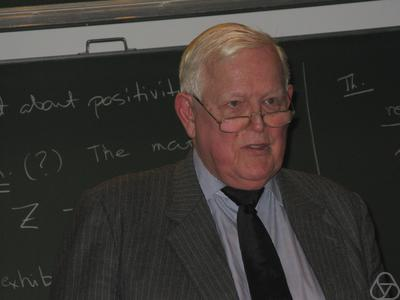
\includegraphics[width=0.75\textwidth]{figs/CONTROLS_portrait_RudolfKalman.jpg}
\end{figure}
\end{frame}


%#####
\section{Introduction}
%#####


\begin{frame}\pw\Large
\frametitle{Kalman Filter/Observer/Estimator}
\framesubtitle{Introduction \tiny cont.}
\begin{figure}
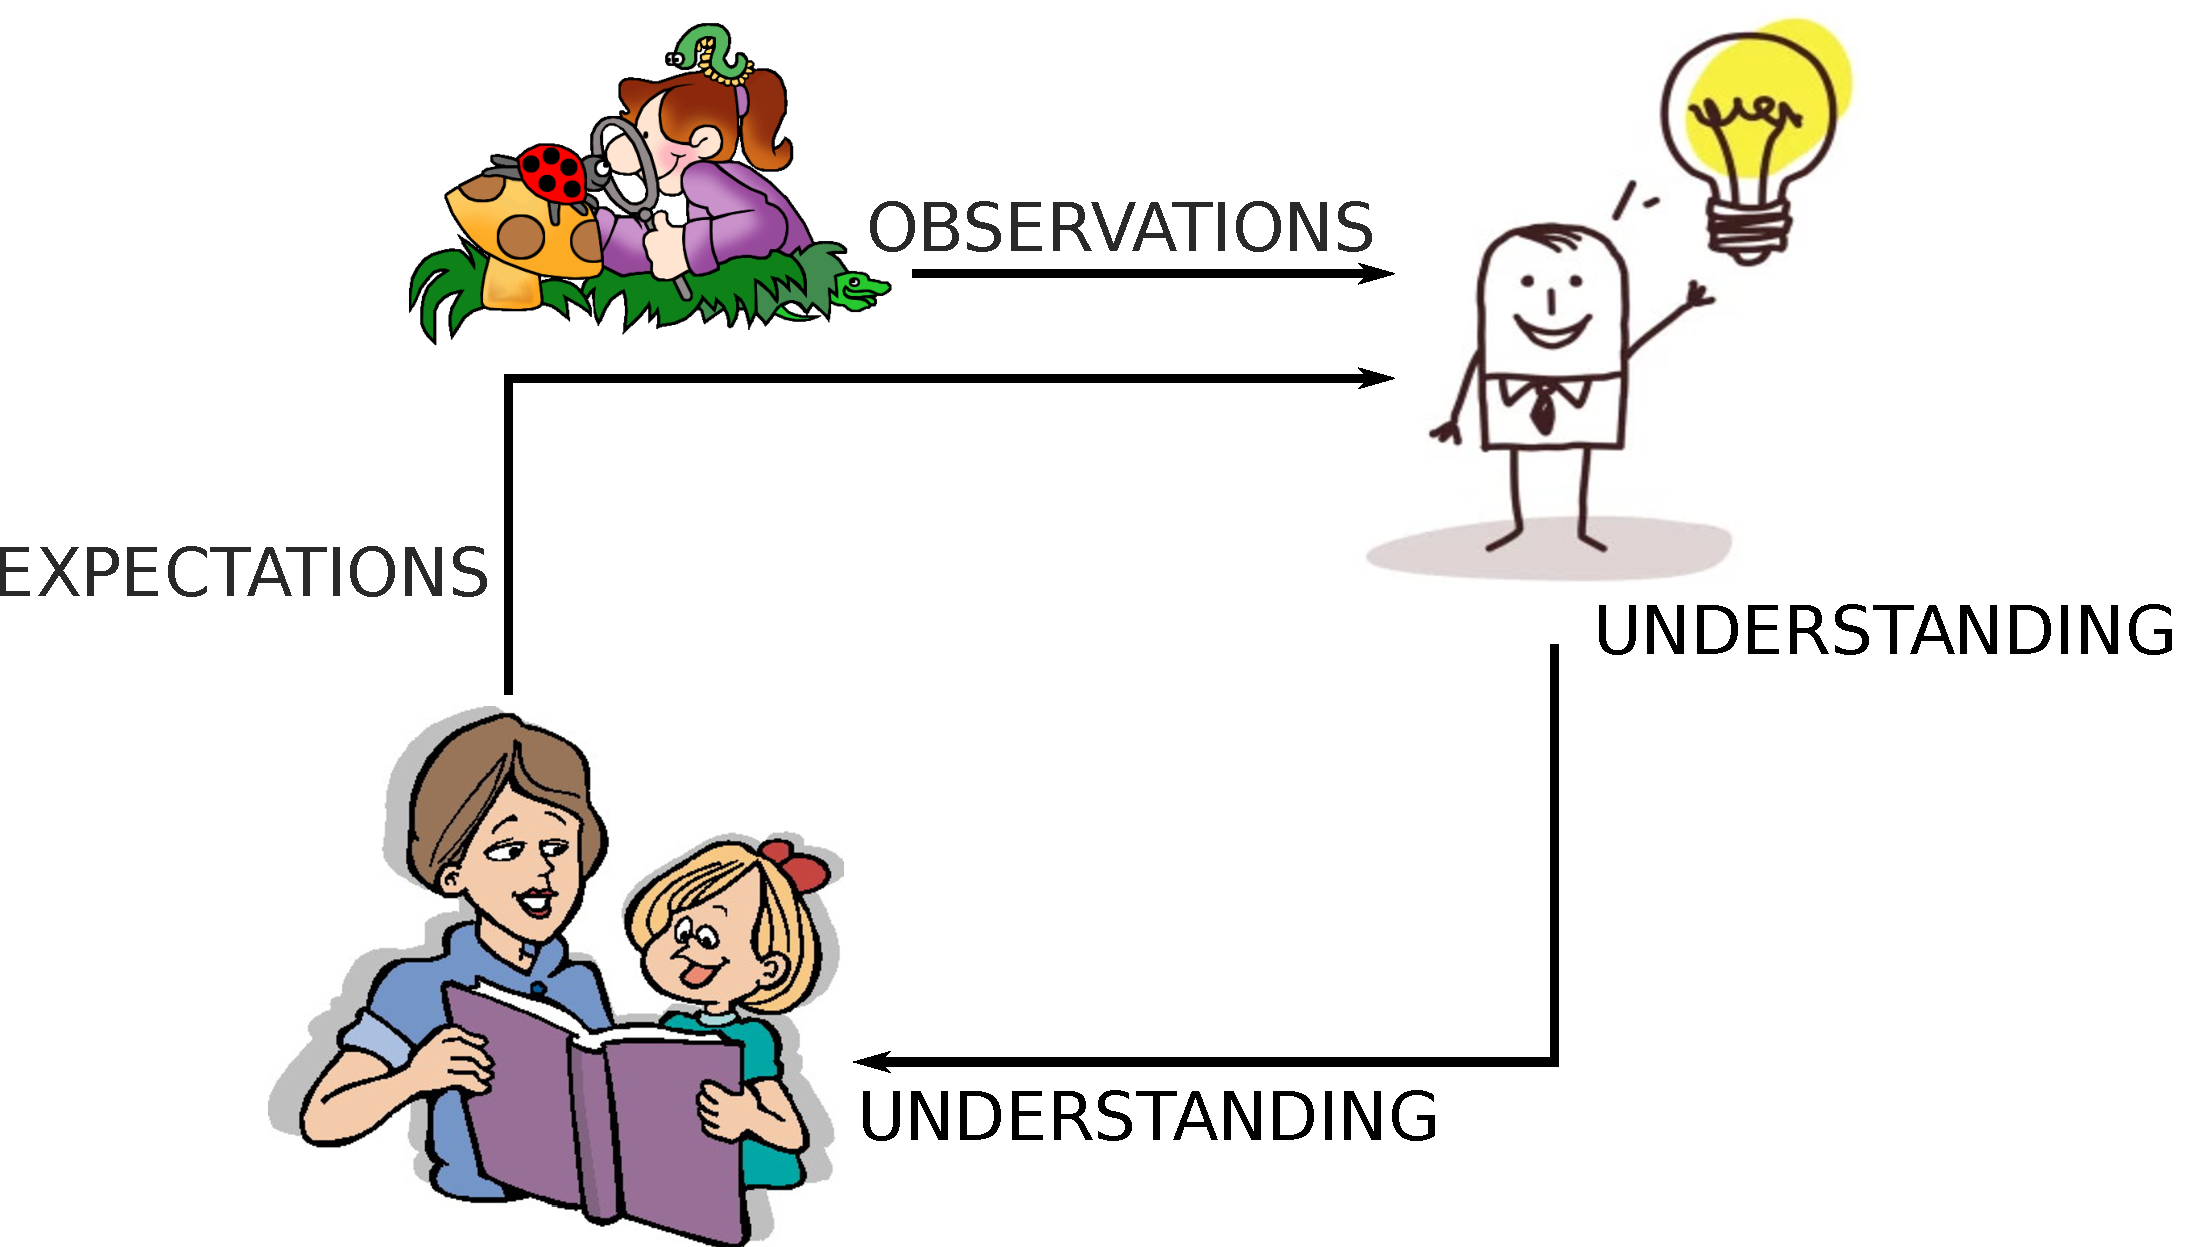
\includegraphics[width=1\textwidth]{figs/WFAR11_UCP_Update_Prediction_BlockDiagram-1.pdf}
\end{figure}
\end{frame}


\begin{frame}\pw\Large
\frametitle{Kalman Filter/Observer/Estimator}
\framesubtitle{Introduction \tiny cont.}
\begin{itemize}
\item \textbf{Bigger picture}
\begin{itemize}\scriptsize
\item The Kalman filter is a type of {\color{blue}Observer}
\item Another name for Observer is Estimator
\end{itemize}
\item \textbf{Goal}
\begin{itemize}\scriptsize
\item The goal of the Kalman filter is to estimate the states of a system
\item The states are represented as $\x$ while the estimated states are represented as $\hat{\x}$
\end{itemize}
\item \textbf{Methodology}
\begin{itemize}\scriptsize
\item Sensors are used to measure the input $u$ and output $y$ of a system
\item The Kalman filter takes an I/O approach, using the input $u$ and output $y$ to estimate what is going on inside the system, i.e., its states $\x$
\item If multiple sensors are used to measure $y$, then the Kalman filter can intelligently combine that information to give a 'good' estimate of the states $\x$
\end{itemize}
\end{itemize}
\end{frame}




%\begin{frame}\pw\Large
%\frametitle{Kalman Filter/Observer/Estimator}
%\framesubtitle{An Observer (Estimator): The Kalman Filter}
%
%\scriptsize
%\begin{itemize}\scriptsize
%\item So, any place that there are sensors to measure the states of a system is a candidate for the Kalman filter
%\item We've already seen that sensors are never accurate
%\item Although the word 'never' should be avoided in engineering, this is one of the places where we can use it
%\item So the job of the Kalman filter is to provide a 'better' estimate of the states of a system than would be obtained with sensors alone
%\end{itemize}
%\end{frame}


%\begin{frame}\pw\Large
%\frametitle{Kalman Filter/Observer/Estimator}
%\framesubtitle{An Observer (Estimator): The Kalman Filter}
%
%\scriptsize
%\begin{itemize}
%\item The true state of the system $\x$ cannot be directly observed, and the Kalman filter provides an algorithm to determine an estimate $\hat{\x}_t$
%\item It does this by combining models of the system and noisy measurements of certain parameters or linear functions of parameters
%\item The estimates of the parameters of interest in the state vector are therefore now provided by probability density functions (pdfs), rather than discrete values
%\item The Kalman filter is based on Gaussian pdfs
%\item To fully describe Gaussian functions, we need to know their variances (1D) and covariances (multiple dimensions) and these are stored in the covariance matrix $\bP$
%\end{itemize}
%\end{frame}



\begin{frame}\pw\Large
\frametitle{Kalman Filter/Observer/Estimator}
\framesubtitle{Introduction \tiny cont.}

\footnotetext{\tiny\hspace{-0.23in} \href{www.cs.cornell.edu/Courses/cs4758/2013sp/materials/MI63slides.pdf‎}{www.cs.cornell.edu/Courses/cs4758/2013sp/materials/MI63slides.pdf‎}}
\begin{itemize}\scriptsize
\item \textbf{Typical uses}
\begin{itemize}\scriptsize
\item Smoothing of noisy data 
\item Providing estimates of parameters of interest
\end{itemize}
\item \textbf{Some applications}
\begin{itemize}\scriptsize
\item GPS receivers
\item PLLs in radio equipment
\item Smoothing the output from laptop trackpads
\item Tracking objects (eg missiles, faces, heads, hands)
\item Economics
\item Navigation
\item Fusing data from radar, laser scanners and stereo-cameras
\item Smart phones
\item Computer games
\item Weather analysis
\end{itemize}
\item The most famous early use of the Kalman filter was in the Apollo navigation computer that took Neil Armstrong to the moon in 1969 and brought him back
\end{itemize}
\end{frame}



\begin{frame}\pw\Large
\frametitle{Kalman Filter/Observer/Estimator}
\framesubtitle{Introduction \tiny cont.}

\footnotetext{\tiny\hspace{-0.23in} \href{http://www.cl.cam.ac.uk/~rmf25/papers/Understanding the Basis of the Kalman Filter.pdf}{Faragher, Ramsey, \emph{Understanding the Basis of the Kalman Filter Via a Simple and Intuitive Derivation}, IEEE Signal Processing Magazine, Sep 2012}}
\scriptsize
\begin{itemize}
\item From a theoretical standpoint, the Kalman filter is an algorithm permitting exact inference in a linear dynamical system, which is a Bayesian model similar to a Hidden Markov Model (HMM) but where the state space of the latent variables is continuous and where all latent and observed variables have a Gaussian distribution (often a multivariate Gaussian distribution)
\item The Kalman filter is based on 5 steps with one equation \\per step:
\begin{enumerate}\scriptsize 
\item {\color{red}Prediction}
\item {\color{red}Prediction uncertainty}
\item Computation of {\color{orange}Kalman gain}
\item {\color{darkgreen}Update} (using {\color{blue}measurement})
\item {\color{darkgreen}Update uncertainty}
\end{enumerate}\scriptsize 
\end{itemize}
\end{frame}

%-------
\subsubsection{1D derivation}
%-------
\begin{frame}\pw\Large
\frametitle{Kalman Filter/Observer/Estimator}
\framesubtitle{Derivation}

\footnotetext{\tiny\hspace{-0.23in} \href{http://www.cl.cam.ac.uk/~rmf25/papers/Understanding the Basis of the Kalman Filter.pdf}{Faragher, Ramsey, \emph{Understanding the Basis of the Kalman Filter Via a Simple and Intuitive Derivation}, IEEE Signal Processing Magazine, Sep 2012}}
\scriptsize
\begin{itemize}
\item The Kalman filter is typically derived using vector algebra as a MMSE (minimum mean squared estimator), an approach suitable for students confident in mathematics but not one that is easy to grasp for students in disciplines that do not require strong mathematics
\end{itemize}
\end{frame}


\begin{frame}\pw\Large
\frametitle{Kalman Filter/Observer/Estimator}
\framesubtitle{Derivation \tiny cont.}
%\footnotetext{\tiny\hspace{-0.23in} \href{http://www.cl.cam.ac.uk/~rmf25/papers/Understanding the Basis of the Kalman Filter.pdf}{Faragher, Ramsey, \emph{Understanding the Basis of the Kalman Filter Via a Simple and Intuitive Derivation}, IEEE Signal Processing Magazine, Sep 2012}}
\begin{itemize}\scriptsize
\item From here on, we focus our attention to a very well written paper on the Kalman filter,   \href{http://www.cl.cam.ac.uk/~rmf25/papers/Understanding the Basis of the Kalman Filter.pdf}{\color{blue} \emph{Understanding the Basis of the Kalman Filter Via a Simple and Intuitive Derivation}} 
\item This paper provides a simple and intuitive derivation of the Kalman filter with the aim of teaching this useful tool to students from disciplines that do not require a strong mathematical background
\item The most complicated level of mathematics required to understand this derivation is the ability to multiply two Gaussian functions together and reduce the result to a compact form
\item In this paper, the Kalman filter is derived from \underline{first principles} considering a simple physical system exploiting a key property of the Gaussian distribution - specifically the property that the product of two Gaussian distributions is another Gaussian distribution [function]
\end{itemize}
\end{frame}



\begin{frame}\pw\Large
\frametitle{Kalman Filter/Observer/Estimator}
\framesubtitle{1D derivation (same units)}

\footnotetext{\tiny\hspace{-0.23in} \href{http://www.cl.cam.ac.uk/~rmf25/papers/Understanding the Basis of the Kalman Filter.pdf}{Faragher, Ramsey, \emph{Understanding the Basis of the Kalman Filter Via a Simple and Intuitive Derivation}, IEEE Signal Processing Magazine, Sep 2012}}
\begin{itemize}\scriptsize 
\item In the following slides, we make two assumptions for the derivation:
\begin{enumerate}\scriptsize 
\item All variables are scalars, i.e., in 1D (an example application is motion along $x$-axis only)
\item The units for prediction, measurement and fused output are all the same
\end{enumerate}
%\item This derivation is in two phases:
%\begin{itemize}\scriptsize 
%\item Phase 1: Units for prediction and measurement are same
%\item Phase 2: Units for prediction and measurement are different
%\end{itemize}
\item An example could be that IMU is used for prediction and GPS is used for measurement
\item The system equation can be modeled as:
\begin{equation*}
\begin{array}{rlllll}
\dot{x}&=&A{\color{Violet}x}+B u+{\color{Aquamarine}w} \ \ \textrm{\tiny (${\color{Aquamarine}w}$ is called process noise)}\\
\end{array}
\end{equation*}
\end{itemize}
\end{frame}



\begin{frame}\pw\Large
\frametitle{Kalman Filter/Observer/Estimator}
\framesubtitle{1D derivation (same units)}

\footnotetext{\tiny\hspace{-0.23in} \href{http://www.cl.cam.ac.uk/~rmf25/papers/Understanding the Basis of the Kalman Filter.pdf}{Faragher, Ramsey, \emph{Understanding the Basis of the Kalman Filter Via a Simple and Intuitive Derivation}, IEEE Signal Processing Magazine, Sep 2012}}
\scriptsize
We have the following variables in the Kalman filter:
\begin{table}\scriptsize
\begin{tabular}{|c |c |l |c |}\hline
\textbf{No}& \textbf{CATEGORY} & \textbf{NAME} & \textbf{SYMBOL}\\\hline
1&INPUT&Input signal & $u$\\\hline
2&PLANT & System Transition Matrix &$A$\\\hline
&" &  Control Input Matrix & $B$\\\hline
&" & Transformation Matrix & $C$\\\hline
3&{\color{blue}SENSOR} &{\color{blue}Measurement mean}&${\color{blue}\mu_2}$\\\hline
&{\color{blue}"} &{\color{blue}Measurement variance}&${\color{blue}\sigma^2_2}$\\\hline
4&OBSERVER &{\color{red}Prediction mean} & ${\color{red}\mu_1}$\\\hline
&" & {\color{red}Prediction variance} & ${\color{red}\sigma^2_1}$\\\hline
&"& {\color{red}Process noise variance}& ${\color{red}Q}$\\\hline
&"&Kalman gain&$K$\\\hline
&" &{\color{darkgreen}Updated mean}& ${\color{darkgreen}\mu_{fused}}$\\\hline
&"&{\color{darkgreen}Updated variance}& ${\color{darkgreen}\sigma^2_{fused}}$\\\hline
\end{tabular}
\end{table}
\end{frame}





\begin{frame}\pw\Large
\frametitle{Kalman Filter/Observer/Estimator}
\framesubtitle{1D derivation (same units) \tiny cont.}

\footnotetext{\tiny\hspace{-0.23in} \href{http://www.cl.cam.ac.uk/~rmf25/papers/Understanding the Basis of the Kalman Filter.pdf}{Faragher, Ramsey, \emph{Understanding the Basis of the Kalman Filter Via a Simple and Intuitive Derivation}, IEEE Signal Processing Magazine, Sep 2012}}
\scriptsize 
Step 1: {\color{red}prediction}\\
\begin{equation*}
\begin{array}{rlllll}
\dot{\hat{x}}&=& A {\color{Violet}\hat{x}}+ B u
\end{array}
\end{equation*}
\end{frame}





\begin{frame}\pw\Large
\frametitle{Kalman Filter/Observer/Estimator}
\framesubtitle{1D derivation (same units) \tiny cont.}

\footnotetext{\tiny\hspace{-0.23in} \href{http://www.cl.cam.ac.uk/~rmf25/papers/Understanding the Basis of the Kalman Filter.pdf}{Faragher, Ramsey, \emph{Understanding the Basis of the Kalman Filter Via a Simple and Intuitive Derivation}, IEEE Signal Processing Magazine, Sep 2012}}
\scriptsize 
Step 2: {\color{red}uncertainty of prediction}
\begin{equation*}
\begin{array}{rlllll}
e=\dot{x} - \dot{\hat{x}}&=&  (A{\color{Violet}x}+B u+{\color{Aquamarine}w}) - (A{\color{Violet}\hat{x}}+B u) \ \ \textrm{\tiny (prediction error)}\\
&=& A\myaa+{\color{Aquamarine}w}\\
\mathrm{COV}[e] &=& E[(e-\mu_e)(e-\mu_e)^T]\ \ \textrm{\tiny (covariance of prediction error)}\\
&=& E[ee^T]\\
&=&E\bigg[\bigg(\dot{x} - \dot{\hat{x}}\bigg)\bigg(\dot{x} - \dot{\hat{x}}\bigg)^T\bigg]\\
&=&E\bigg[\bigg(  A\myaa+{\color{Aquamarine}w}\bigg)\bigg(  A\myaa+{\color{Aquamarine}w}\bigg)^T\bigg]\\
&=&E\bigg[\bigg(  A\myaa+{\color{Aquamarine}w}\bigg)\bigg(  \big(A\myaa\big)^T+{\color{Aquamarine}w}^T\bigg)\bigg]\\
&=&E\bigg[\bigg(  A\myaa+{\color{Aquamarine}w}\bigg)\bigg( \myaa^T A^T+{\color{Aquamarine}w}^T\bigg)\bigg]\\
&=&E\bigg[ A\myaa\myaa^T A^T +  A\myaa {\color{Aquamarine}w}^T \\
&&+ {\color{Aquamarine}w}\myaa^T A^T + {\color{Aquamarine}w}{\color{Aquamarine}w}^T\bigg]\\
&=& A E[\myaa\myaa^T] A^T + E[{\color{Aquamarine}w}{\color{Aquamarine}w}^T]\\
&=& A\varfused A^T +Q\\
&=& A^2\varfused +Q
\end{array}
\end{equation*}
\end{frame}



\begin{frame}\pw\Large
\frametitle{Kalman Filter/Observer/Estimator}
\framesubtitle{1D derivation (same units) \tiny cont.}

\footnotetext{\tiny\hspace{-0.23in} \href{http://www.cl.cam.ac.uk/~rmf25/papers/Understanding the Basis of the Kalman Filter.pdf}{Faragher, Ramsey, \emph{Understanding the Basis of the Kalman Filter Via a Simple and Intuitive Derivation}, IEEE Signal Processing Magazine, Sep 2012}}
\scriptsize
Steps 3 and 4: {\color{orange}Kalman gain} and {\color{darkgreen}update}\\
The mean $\mufused$ of the Gaussian function obtained when \\two Gaussian distributions with mean and variance $\muone$, $\varone$\\ and $\mutwo$, $\vartwo$ respectively are multiplied is given by,
\begin{equation*}
\begin{array}{rlllllll}
\mufused &=& \frac { \muone \vartwo + \mutwo \varone }{\varone + \vartwo}\\
&=&\muone + \frac{\varone(\mutwo-\muone)}{\varone + \vartwo}&=&\muone  + {\color{Orange}k_1}(\mutwo-\muone)\\
&=&\mutwo + \frac{\vartwo(\muone-\mutwo)}{\varone + \vartwo}&=&\mutwo  + {\color{Orange}k_2}(\muone-\mutwo)
\end{array}
\end{equation*}
where ${\color{Orange}k_1}=\frac{\varone}{\varone + \vartwo}$ and ${\color{Orange}k_2}=\frac{\vartwo}{\varone + \vartwo}$
\begin{itemize}\scriptsize
\item Notice that ${\color{Orange}k_1}$ and ${\color{Orange}k_2}$ are always positive fractions
\item The mean $\mufused$ is obtained by:
\begin{itemize}\scriptsize
\item offsetting $\muone$ with the weighted difference of $\mutwo-\muone$, or 
\item offsetting $\mutwo$ with the weighted difference of $\muone-\mutwo$
\end{itemize}
\item It is more common to see 
$\mufused=\muone  + {\color{Orange}k_1}(\mutwo-\muone)$ than to see $\mufused=\mutwo  + {\color{Orange}k_2}(\muone-\mutwo)$ although of course, both are correct
\end{itemize}
\end{frame}



\begin{frame}\pw\Large
\frametitle{Kalman Filter/Observer/Estimator}
\framesubtitle{1D derivation (same units) \tiny cont.}

\footnotetext{\tiny\hspace{-0.23in} \href{http://www.cl.cam.ac.uk/~rmf25/papers/Understanding the Basis of the Kalman Filter.pdf}{Faragher, Ramsey, \emph{Understanding the Basis of the Kalman Filter Via a Simple and Intuitive Derivation}, IEEE Signal Processing Magazine, Sep 2012}}
\scriptsize
Step 5: {\color{darkgreen}uncertainty of update}\\
The variance $\varfused$ of the Gaussian function obtained when\\ two Gaussian distributions with mean and variance $\muone$, $\varone$\\ and $\mutwo$, $\vartwo$ respectively are multiplied is given by,
\begin{equation*}
\begin{array}{rlllllll}
\varfused
&=& \frac{\varone \vartwo}{\varone + \vartwo}\\
&=&\varone - \frac{\color{red}\sigma^4_1}{\varone + \vartwo}
&=&\varone-\frac{\varone}{\varone + \vartwo}\varone
&=&(1-{\color{Orange}k_1})\varone\\
&=&\vartwo - \frac{\color{blue}\sigma^4_2}{\varone + \vartwo}
&=&\vartwo-\frac{\vartwo}{\varone + \vartwo}\vartwo
&=&(1-{\color{Orange}k_2})\vartwo
\end{array}
\end{equation*}
where ${\color{Orange}k_1}$ and ${\color{Orange}k_2}$ are the same as defined in the previous slide
\begin{itemize}\scriptsize
\item Since ${\color{Orange}k_1}$ and ${\color{Orange}k_2}$ are always positive fractions, the variance $\varfused$ of the output Gaussian function is always less than $\varone$ and $\vartwo$
\item In other words, multiplying two Gaussians decreases the variance of the resulting Gaussian to less than the variances of the input Gaussians
\item It is more common to see $\varfused=(1-{\color{Orange}k_1})\varone$ than to see $\varfused=(1-{\color{Orange}k_2})\vartwo$ although of course, both are correct
\end{itemize}
\end{frame}


\begin{frame}\pw\Large
\frametitle{Kalman Filter/Observer/Estimator}
\framesubtitle{1D derivation (different units)}

\footnotetext{\tiny\hspace{-0.23in} \href{http://www.cl.cam.ac.uk/~rmf25/papers/Understanding the Basis of the Kalman Filter.pdf}{Faragher, Ramsey, \emph{Understanding the Basis of the Kalman Filter Via a Simple and Intuitive Derivation}, IEEE Signal Processing Magazine, Sep 2012}}
\scriptsize 
\begin{itemize}\scriptsize
\item Now, we assume that the units of the prediction \\and fused output are the same while the units of the measurement are different
\item However, we want all units to be the same as for the measurement
\item Assume that the conversion can be obtained by multiplying with the factor $C$
\item We now repeat the previous derivation using this unit conversion
\end{itemize}
\end{frame}



\begin{frame}\pw\Large
\frametitle{Kalman Filter/Observer/Estimator}
\framesubtitle{1D derivation (different units) \tiny cont.}

\footnotetext{\tiny\hspace{-0.23in} \href{http://www.cl.cam.ac.uk/~rmf25/papers/Understanding the Basis of the Kalman Filter.pdf}{Faragher, Ramsey, \emph{Understanding the Basis of the Kalman Filter Via a Simple and Intuitive Derivation}, IEEE Signal Processing Magazine, Sep 2012}}
\scriptsize 
Step 1: {\color{red}prediction}\\
Same as before
\end{frame}


\begin{frame}\pw\Large
\frametitle{Kalman Filter/Observer/Estimator}
\framesubtitle{1D derivation (different units) \tiny cont.}

\footnotetext{\tiny\hspace{-0.23in} \href{http://www.cl.cam.ac.uk/~rmf25/papers/Understanding the Basis of the Kalman Filter.pdf}{Faragher, Ramsey, \emph{Understanding the Basis of the Kalman Filter Via a Simple and Intuitive Derivation}, IEEE Signal Processing Magazine, Sep 2012}}
\scriptsize 
Step 2: {\color{red}uncertainty of prediction}\\
Same as before
\end{frame}


\begin{frame}\pw\Large
\frametitle{Kalman Filter/Observer/Estimator}
\framesubtitle{1D derivation (different units) \tiny cont.}

\scriptsize
\footnotetext{\tiny\hspace{-0.23in} \href{http://www.cl.cam.ac.uk/~rmf25/papers/Understanding the Basis of the Kalman Filter.pdf}{Faragher, Ramsey, \emph{Understanding the Basis of the Kalman Filter Via a Simple and Intuitive Derivation}, IEEE Signal Processing Magazine, Sep 2012}}\scriptsize
Steps 3 and 4: {\color{orange}Kalman gain} and {\color{darkgreen}update}\\
We convert the prediction and fused output units to measurement units as follows,

\begin{equation*}
\begin{array}{rlllllll}
C\mufused &= \frac { C\muone \vartwo + \mutwo C^2\varone }{C^2\varone + \vartwo}\\\\
\Rightarrow \mufused &= \frac { \muone \vartwo + \mutwo C\varone }{C^2\varone + \vartwo}\\\\
&=\muone + \frac{\varone(C\mutwo-C^2\muone)}{C^2\varone + \vartwo}=\muone + \frac{C\varone(\mutwo-C\muone)}{C^2\varone + \vartwo} =\muone  + {\color{Orange}K}(\mutwo-C\muone)
\end{array}
\end{equation*}

where ${\color{Orange}K}=\frac{C\varone}{C^2\varone + \vartwo}$
\begin{itemize}\scriptsize
%\item Notice that ${\color{Orange}K}$ is always a positive fraction
\item The mean $\mufused$ is obtained by offsetting $\muone$ with the weighted difference of $\mutwo-C\muone$
\item This weighting ${\color{Orange}K}$ is called the Kalman gain
\end{itemize}
\end{frame}



\begin{frame}\pw\Large
\frametitle{Kalman Filter/Observer/Estimator}
\framesubtitle{1D derivation (different units) \tiny cont.}

\footnotetext{\tiny\hspace{-0.23in} \href{http://www.cl.cam.ac.uk/~rmf25/papers/Understanding the Basis of the Kalman Filter.pdf}{Faragher, Ramsey, \emph{Understanding the Basis of the Kalman Filter Via a Simple and Intuitive Derivation}, IEEE Signal Processing Magazine, Sep 2012}}
\scriptsize
Step 5: {\color{darkgreen}uncertainty of update}\\
We convert the prediction and fused output units to measurement units as follows,
\begin{equation*}
\begin{array}{rlllllll}
C^2 \varfused&=& \frac{C^2\varone \vartwo}{C^2\varone + \vartwo}\\\\
\Rightarrow \varfused&=& \frac{\varone \vartwo}{C^2\varone + \vartwo}\\\\
&=&\varone - \frac{C^2\color{red}\sigma^4_1}{C^2\varone + \vartwo}
&=\varone-\frac{C\varone}{C^2\varone + \vartwo}C\varone
&=(1-{\color{Orange}K}C)\varone\\\\
\end{array}
\end{equation*}
where ${\color{Orange}K}$ is the Kalman gain as defined in the previous slide
%\begin{itemize}\scriptsize
%\item Since ${\color{Orange}k_1}$ and ${\color{Orange}k_2}$ are always positive fractions, the variance $\varfused$ of the output Gaussian function is always less than $\varone$ and $\vartwo$
%\item In other words, multiplying two Gaussians decreases the variance of the resulting Gaussian to less than the variances of the input Gaussians
%\end{itemize}
\end{frame}



\begin{frame}[plain]\pw\Large
\frametitle{Kalman Filter/Observer/Estimator}
\framesubtitle{1D derivation (different units) \tiny cont.}

\footnotetext{\tiny\hspace{-0.23in} \href{http://www.cl.cam.ac.uk/~rmf25/papers/Understanding the Basis of the Kalman Filter.pdf}{Faragher, Ramsey, \emph{Understanding the Basis of the Kalman Filter Via a Simple and Intuitive Derivation}, IEEE Signal Processing Magazine, Sep 2012}}
\scriptsize
So, in summary, the equations are:
%\footnotetext{\tiny\hspace{-0.23in} \hspace{-0.24in}- \href{http://en.wikipedia.org/wiki/Kalman_filter}{http://en.wikipedia.org/wiki/Kalman\_filter}\\
%- \href{http://blog.jafma.net/2010/11/09/the-product-of-two-Gaussian-pdfs-is-not-a-pdf-but-is-Gaussian-a-k-a-loving-algebra/}{http://blog.jafma.net/2010/11/09/the-product-of-two-Gaussian-pdfs-is-not-a-pdf-but-is-Gaussian-a-k-a-loving-algebra/}}

\begin{figure}[h]
\centering
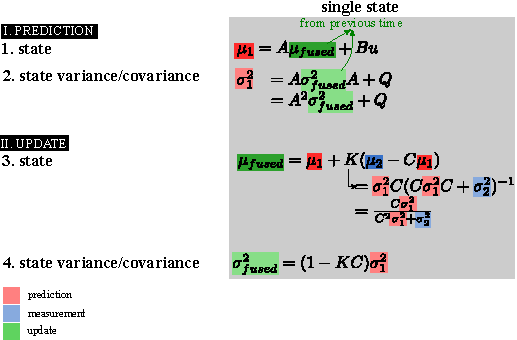
\includegraphics[width=0.9\textwidth]{figs/TRK_KalmanFilter_equations-1D.pdf}
\end{figure}
\begin{itemize}\scriptsize
\item The predicted state is ${\color{red}\mu_1}$ and its variance is ${\color{red}\sigma^2_1}$
\item The measurement (observation) is ${\color{blue}\mu_2}$ and its variance is ${\color{blue}\sigma^2_2}$
\item The prediction and measurement are combined using the Kalman gain $K$ (should be called $L$ but we've used $K$ since all books call it $K$) to get the updated state ${\color{darkgreen}\mu_{fused}}$ and its variance ${\color{darkgreen}\sigma^2_{fused}}$
\end{itemize}

\end{frame}



\begin{frame}\pw\Large
\frametitle{Kalman Filter/Observer/Estimator}
\framesubtitle{1D derivation (different units) \tiny cont.}

\begin{itemize}\scriptsize
\item \underline{Step 1}: The future state is predicted according to the\\ system model (or through a sensor)
\item \underline{Step 2}: If a random variable is multiplied with a constant $A$, then the resulting variance is multiplied with constant $A^2$.  In addition, the resulting variance is increased by $Q$, i.e., we have added more uncertainty.
\item \underline{Step 3}: The Kalman gain is computed.  This is the gain of the observer and although we use $K$, this is actually $L$.  Also notice that,
\begin{equation*}
\begin{array}{rlllll}
K&=\frac{C\sigma_1^2}{C^2\sigma_1^2+\sigma_2^2}\\
\Rightarrow \frac{KC^2}{C}&=\frac{\sigma_1^2}{\sigma_1^2+\frac{1}{C^2}\sigma_2^2}\\
\Rightarrow KC&=\frac{\sigma_1^2}{\sigma_1^2+\frac{1}{C^2}\sigma_2^2} <1\\
\Rightarrow \sigma^2_{fused}&<\sigma^2_1
\end{array}
\end{equation*}
\item \underline{Step 4}: The difference between actual and expected observation is weighted by $K$ and added to our predicted estimate
\item \underline{Step 5}: The variance of the update decreases from $\sigma^2_1$ to $(1-KC)\sigma^2_1$, a key strength of the Kalman filter !  Also, if $\sigma^2_1$ goes up, so does K.  But, if $\sigma^2_2$ goes up, K goes down.  
\end{itemize}
\end{frame}



%-------
\subsubsection{1D example}
%-------

\begin{frame}[plain]\pw\Large
\frametitle{Kalman Filter/Observer/Estimator}
\framesubtitle{1D example}

\footnotetext{\tiny\hspace{-0.23in} \href{http://www.cl.cam.ac.uk/~rmf25/papers/Understanding the Basis of the Kalman Filter.pdf}{Faragher, Ramsey, \emph{Understanding the Basis of the Kalman Filter Via a Simple and Intuitive Derivation}, IEEE Signal Processing Magazine, Sep 2012}}
\scriptsize

\begin{itemize}\scriptsize
\item \textbf{Introduction}
\begin{itemize}\scriptsize
\item We start by considering a simple 1-D problem, i.e., we have only one state
\item We have a train moving along a railway line, as shown below
\end{itemize}
\item \textbf{Goal}
\begin{itemize}\scriptsize
\item The goal is for an onboard computer to correctly estimate the position of the train
\end{itemize}
\begin{figure}[h]
\centering
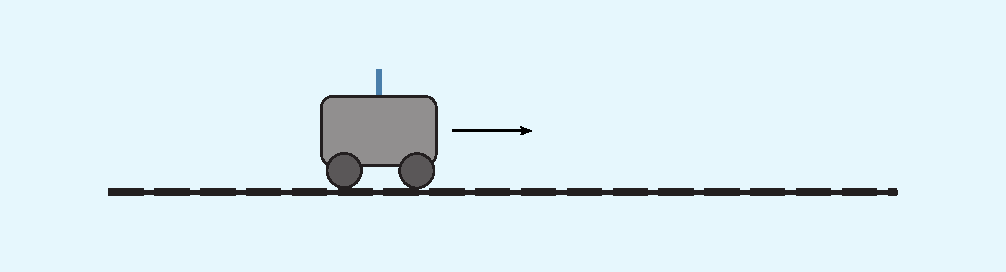
\includegraphics[width=1.35\textwidth]{figs/2012_MAG_Understanding_the_Basis_of_the_Kalman_Filter_fig0.pdf}
\end{figure}
%\item The state vector $\x_t$ contains the position and velocity of the train
%\begin{equation*}
%\x_t = 
%\begin{bmatrix}
%x_t\\
%\dot{x}_t
%\end{bmatrix}
%\end{equation*}
\end{itemize}

\end{frame}




%#####
\section{A Naive Start}
%#####



%#####
\section{Observing and Experiencing}
%#####


%#####
\section{We Are Wiser}
%#####

\begin{frame}[plain]\pw\Large
\frametitle{Kalman Filter/Observer/Estimator}
\framesubtitle{1D example \tiny cont.}

\footnotetext{\tiny\hspace{-0.23in} \href{http://www.cl.cam.ac.uk/~rmf25/papers/Understanding the Basis of the Kalman Filter.pdf}{Faragher, Ramsey, \emph{Understanding the Basis of the Kalman Filter Via a Simple and Intuitive Derivation}, IEEE Signal Processing Magazine, Sep 2012}}
\scriptsize

\begin{enumerate}\scriptsize
\item \textbf{Input}: The train driver may apply a \emph{braking} or \emph{accelerating} input to the train
\item \textbf{Plant (System)}: Since we have only one state, position of the train along the x axis, we use a single state model, $x[k]=Ax[k-1]+Bu[k-1]$
\item \textbf{Sensor}: The train can get distance measurements from a radio ranging system (similar to Distance Measuring Equipment, DME, in aircraft)
\item \textbf{Compensator}:
\begin{itemize}\scriptsize
\item \textbf{Controller}: None 
\item \textbf{Observer}: Kalman filter
\end{itemize}
\end{enumerate}
\begin{figure}[h]
\centering
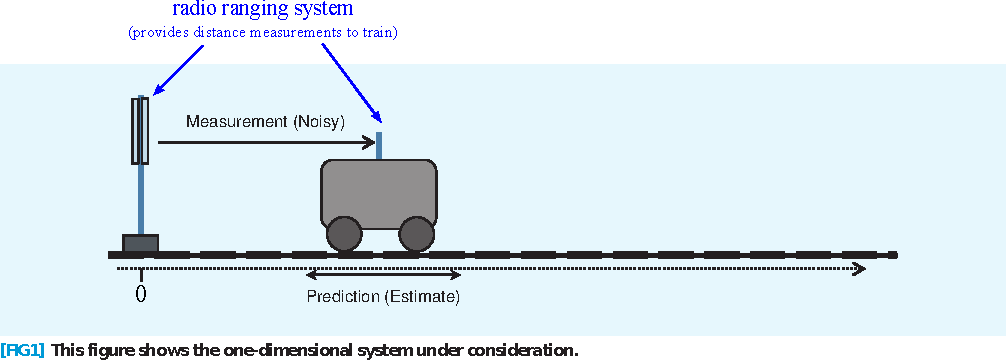
\includegraphics[width=1.35\textwidth]{figs/2012_MAG_Understanding_the_Basis_of_the_Kalman_Filter_fig1.pdf}
\end{figure}

\end{frame}









%\begin{frame}\pw\Large
%\frametitle{Kalman Filter/Observer/Estimator}
%\framesubtitle{An Observer (Estimator): The Kalman Filter}
%
%\scriptsize
%\begin{itemize}
%\item The Kalman filter algorithm involves two stages: prediction and measurements update
%\begin{equation*}\scriptsize
%\begin{array}{rllllllll}
%\xh_{t|t-1} &=& \F_t \xh_{t-1|t-1} + \B_t \bu_t\\
%\bP_{t|t-1} &=& \F_t\bP_{t-1|t-1}\F_t^T + \Q_t
%\end{array}
%\end{equation*}
%where $ \Q_t$ is the process noise covariance matrix associated with noisy control inputs
%\end{itemize}
%\end{frame}





\begin{frame}[plain]\pw\Large
\frametitle{Kalman Filter/Observer/Estimator}
\framesubtitle{1D example \tiny cont.}

\footnotetext{\tiny\hspace{-0.23in} \href{http://www.cl.cam.ac.uk/~rmf25/papers/Understanding the Basis of the Kalman Filter.pdf}{Faragher, Ramsey, \emph{Understanding the Basis of the Kalman Filter Via a Simple and Intuitive Derivation}, IEEE Signal Processing Magazine, Sep 2012}}
\scriptsize

\underline{\textbf{Initialization}}
\begin{itemize}\scriptsize
\item At some initial time, we have some idea of where the train is
\item This idea is represented by a Gaussian distribution (green curve below)
\item At places where the Gaussian distribution has high amplitude, we have more confidence
\item Therefore, most likely, the train is at $\mu_{fused}$
\item The bigger that $\sigma_{fused}^2$ is, the more spread the Gaussian distribution, and the less our confidence of where the train really is
\end{itemize}
\begin{figure}[h]
\centering
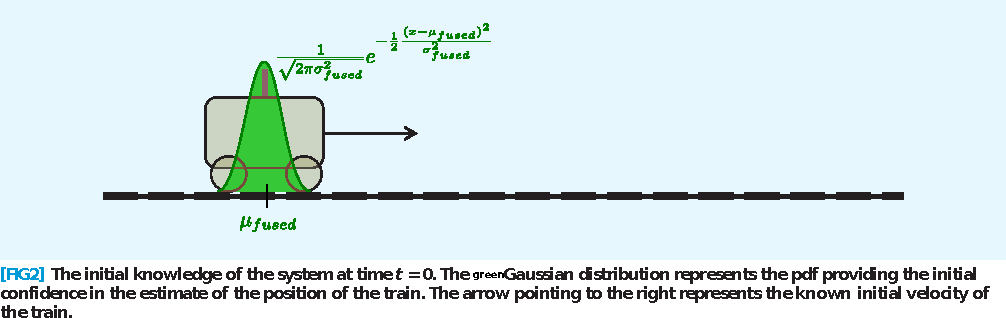
\includegraphics[width=1.35\textwidth]{figs/2012_MAG_Understanding_the_Basis_of_the_Kalman_Filter_fig2_mine.pdf}
\end{figure}

\end{frame}


\begin{frame}[plain]\pw\Large
\frametitle{Kalman Filter/Observer/Estimator}
\framesubtitle{1D example \tiny cont.}

\footnotetext{\tiny\hspace{-0.23in} \href{http://www.cl.cam.ac.uk/~rmf25/papers/Understanding the Basis of the Kalman Filter.pdf}{Faragher, Ramsey, \emph{Understanding the Basis of the Kalman Filter Via a Simple and Intuitive Derivation}, IEEE Signal Processing Magazine, Sep 2012}}
\scriptsize

\underline{\textbf{Step 1 of the Kalman Filter: prediction}}
\begin{itemize}\scriptsize
\item Now, we will predict the new position of the train
\item The Gaussian is now more spread
\item Our maximum belief is in the train being at {\color{red}$\mu_1$}
\end{itemize}
\begin{figure}[h]
\centering
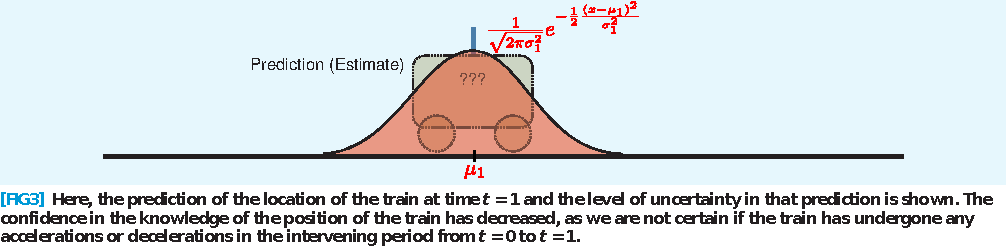
\includegraphics[width=1.35\textwidth]{figs/2012_MAG_Understanding_the_Basis_of_the_Kalman_Filter_fig3.pdf}
\end{figure}

\end{frame}


\begin{frame}[plain]\pw\Large
\frametitle{Kalman Filter/Observer/Estimator}
\framesubtitle{1D example \tiny cont.}

\footnotetext{\tiny\hspace{-0.23in} \href{http://www.cl.cam.ac.uk/~rmf25/papers/Understanding the Basis of the Kalman Filter.pdf}{Faragher, Ramsey, \emph{Understanding the Basis of the Kalman Filter Via a Simple and Intuitive Derivation}, IEEE Signal Processing Magazine, Sep 2012}}
\scriptsize

\underline{\textbf{Intermediate step: measurement arrives}}
\begin{itemize}\scriptsize
\item Now, we get a measurement from the radio ranging system, which is also noisy
\item According to the radio ranging system, the train is most likely at  $\mu_2$
\item Now, we have to combine the prediction (red Gaussian) with the measurement (blue Gaussian) to come to a more intelligent decision
\item This is known as \emph{sensor fusion}
\end{itemize}
\begin{figure}[h]
\centering
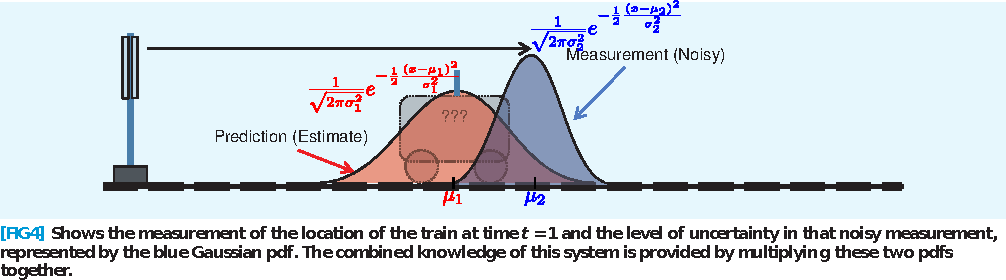
\includegraphics[width=1.35\textwidth]{figs/2012_MAG_Understanding_the_Basis_of_the_Kalman_Filter_fig4.pdf}
\end{figure}

\end{frame}


\begin{frame}[plain]\pw\Large
\frametitle{Kalman Filter/Observer/Estimator}
\framesubtitle{1D example \tiny cont.}

\footnotetext{\tiny\hspace{-0.23in} \href{http://www.cl.cam.ac.uk/~rmf25/papers/Understanding the Basis of the Kalman Filter.pdf}{Faragher, Ramsey, \emph{Understanding the Basis of the Kalman Filter Via a Simple and Intuitive Derivation}, IEEE Signal Processing Magazine, Sep 2012}}
\scriptsize

\underline{\textbf{Step 2 of the Kalman Filter: update}}
\begin{itemize}\scriptsize
\item We combine the prediction Gaussian (red) with the measurement Gaussian (blue) by multiplying them
\item This gives us the green Gaussian
\item We call the peak of the green Gaussian ${\color{darkgreen}\mu_{fused}}$
\item So, we have decided that the train is most likely at ${\color{darkgreen}\mu_{fused}}$, but of course we're not sure, and that unsurety is shown by the green Gaussian
\item Notice that the green Gaussian is less spread than the red Gaussian or the blue Gaussian showing that we are more sure now than before of the position of the train
\end{itemize}
\begin{figure}[h]
\centering
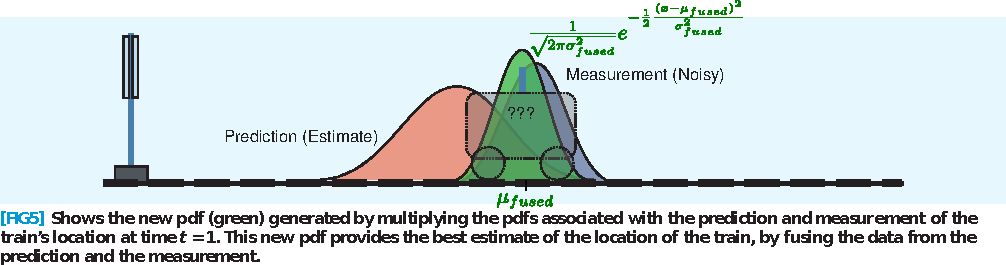
\includegraphics[width=1.35\textwidth]{figs/2012_MAG_Understanding_the_Basis_of_the_Kalman_Filter_fig5.pdf}
\end{figure}

\end{frame}


\begin{frame}[fragile]\pw\Large
\frametitle{Kalman Filter/Observer/Estimator}
\framesubtitle{1D example \tiny cont.}

\scriptsize
The code below implements 2 time steps for the train:
\tinyvvv \begin{lstlisting}[language=Matlab]
clear;clc;clf;

%initialization
x           =   -5:0.1:25;  %x axis
A           =   2;          %state transition matrix
B           =   5;          %control input matrix
C           =   1;          %transformation matrix
u           =   1;          %control input
Q           =   1.2;        %process noise variance, adds uncertainty to prediction
mu_2        =   [7 14];     %the output of the radio ranging system at next two times
var_2       =   1;          %the variance of the radio ranging system given by manufacturer

mu_f        =   0;          %the estimated location of the train at current time, k=0
var_f       =   1;          %the estimated variance of our estimate at current time, k=0

pdf_0       =   (1/sqrt(2*pi*var_f))*exp(-(0.5/var_f)*(x-mu_f).^2);


%=====================================
%run Kalman Filter
%=====================================
for k=1:2
    %predict
    mu_1        =   A*mu_f      +   B*u;
    var_1       =   A^2*var_f   +   Q;
    %update
    K           =   (C*var_1)/(C^2*var_1 + var_2);
    mu_f        =   mu_1 + K*(mu_2(k)-C*mu_1);
    var_f       =   (1-K*C)*var_1;
    
    pred        =   (1/sqrt(2*pi*var_1))*exp(-(0.5/var_1)*(x-mu_1).^2);
    meas        =   (1/sqrt(2*pi*var_2))*exp(-(0.5/var_2)*(x-mu_2(k)).^2);
    fused       =   (1/sqrt(2*pi*var_f))*exp(-(0.5/var_f)*(x-mu_f).^2);
    
                    axis([-5 25 0 0.5]); 
                    grid on;
                    hold on;


                    plot(x,pred, 'r--x');
                    plot(x,meas, 'b--o');
                    plot(x,fused,'g--.')
                    plot(x,pdf_0,'g--.');                    
end
legend('predicted', 'measured', 'fused')
xlabel('railway track (meters), direction along which train is traveling ->')
ylabel('belief in fused/predicted/measured position of train')
title('Data fusion using the Kalman Filter')
\end{lstlisting}
\end{frame}








\begin{frame}\pw\Large
\frametitle{Kalman Filter/Observer/Estimator}
\framesubtitle{1D example \tiny cont.}

\scriptsize The code on the previous slide produces this output:
\begin{figure}[h]
\centering
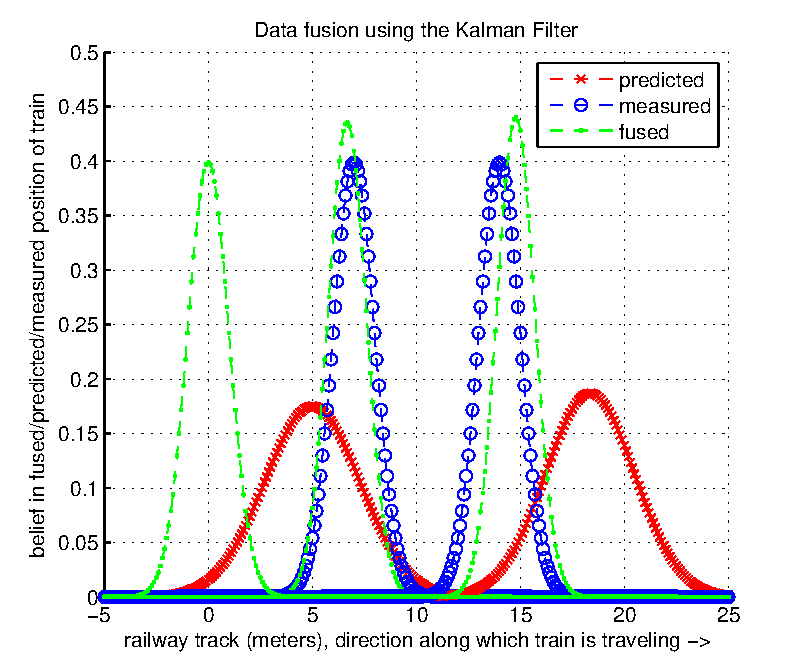
\includegraphics[width=0.7\textwidth]{figs/CONTROLS_Kalman_train_example.pdf}
\caption{\tiny In this example, a train is moving along the x-axis.  The problem begins at time $kT=0$ sec when our initial estimate of the train is that it is standing at $x=0$ meters.  The prediction and measurements for the next two time instants, $kT=1$ sec and $kT=2$ sec are shown.  We assume for simplicity but without loss of generality, that $T=1$~sec, and therefore we use $k$ (in sec) to depict time.  It may be mentioned that the version of the Kalman filter for continuous time is called the Kalman-Bucy filter.}
\end{figure}
\end{frame}






%-------
\subsubsection{Multiple-D derivation}
%-------
\begin{frame}[plain]\pw\Large
\frametitle{Kalman Filter/Observer/Estimator}
\framesubtitle{Multiple-D derivation}

\footnotetext{\tiny\hspace{-0.23in} \hspace{-0.24in} \href{http://en.wikipedia.org/wiki/Kalman_filter}{http://en.wikipedia.org/wiki/Kalman\_filter}}

\begin{itemize}\scriptsize
\item Now, let's take a look at the Kalman Filter when more than one state is involved
\item Notice the one-to-one correspondence between equations in 1D (i.e. one state) and multiple states
\end{itemize}
\begin{figure}[h]
\centering
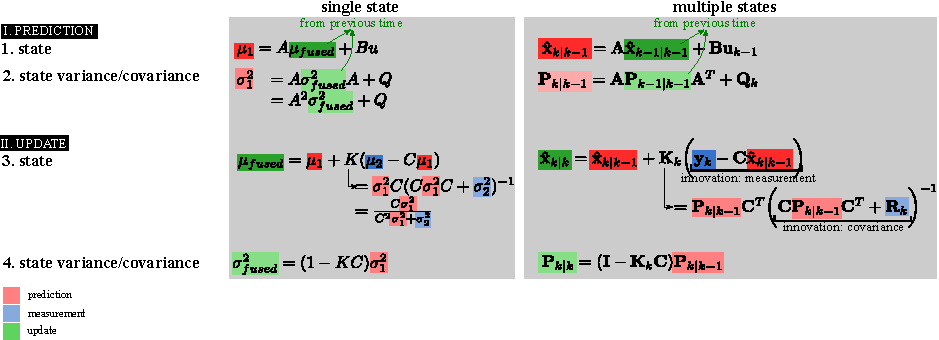
\includegraphics[width=1.4\textwidth]{figs/TRK_KalmanFilter_equations-2D.pdf}
\end{figure}

\end{frame}


%-------
\subsubsection{2D example}
%-------


\begin{frame}[plain]\pw\Large
\frametitle{Kalman Filter/Observer/Estimator}
\framesubtitle{2D example}


\scriptsize
\begin{itemize}
\item In the single state example, we used the Kalman filter to fuse, i.e., combine two\\ pieces of information: first, our prediction of the position of a train, and second,\\ the measurement of the train's position obtained from a radio ranging system.  The result of our fusion was an estimate of the train's position.
\item Now, we will extend the Kalman Filter to 2 states (also called 2 dimensions, or 2D), i.e., we will focus on a car that moves in the xy-plane and not just in a straight line along the x-axis like a train
\item Here is an example in 2D followed by its code on the next 3 slides
\end{itemize}
\vspace{-0.18in}
\begin{figure}[h]
\centering
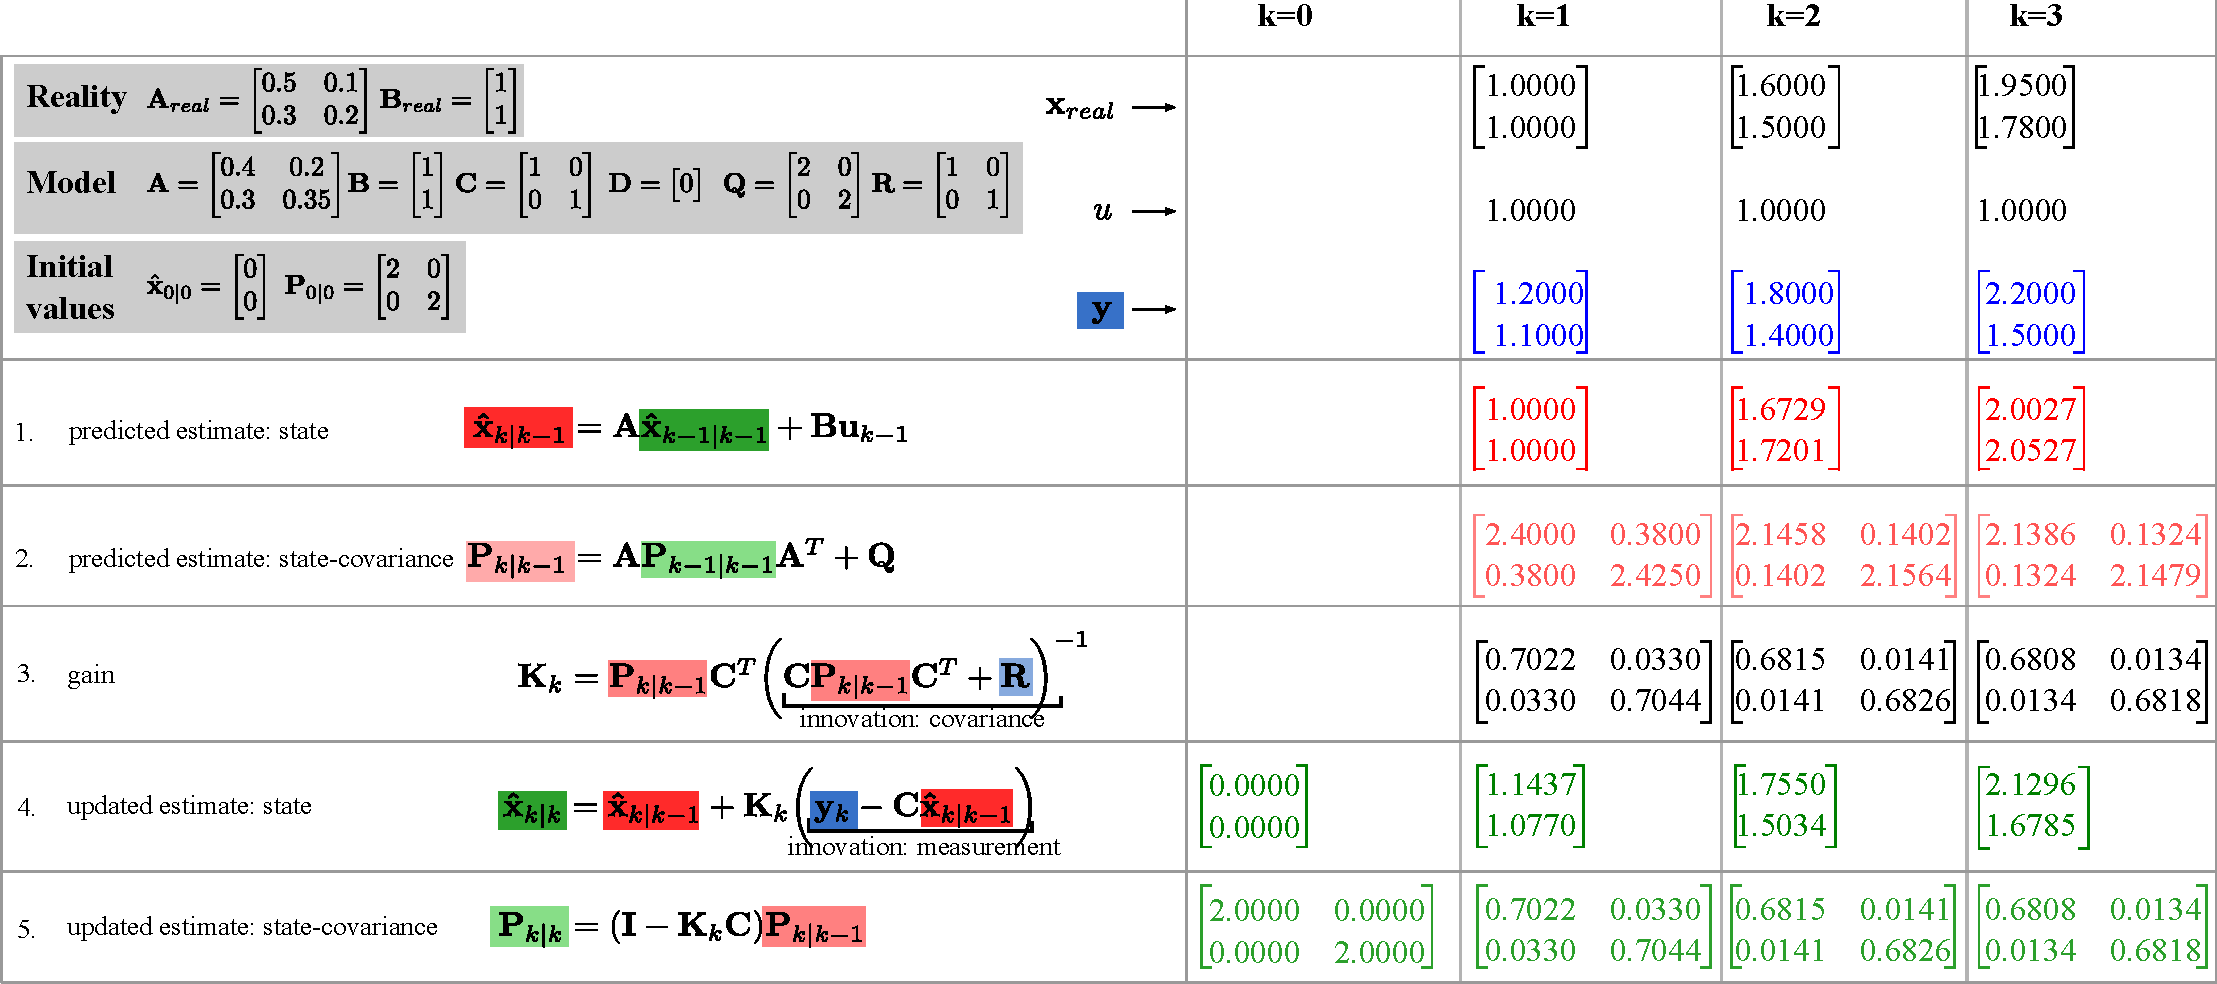
\includegraphics[width=1.4\textwidth]{figs/TRK_KalmanFilter_example.pdf}
\end{figure}

\end{frame}



\begin{frame}[fragile]\pw\Large
\frametitle{Kalman Filter/Observer/Estimator}
\framesubtitle{2D example \tiny cont.}

%\hspace{-0.2in}\begin{itemize}\scriptsize
%\item The code below implements 2 time steps for the train
%\end{itemize}
\tinyvvv \begin{lstlisting}[language=Matlab]
%%%%%%%%%%%%%%%%%%%%%%%%%%%%%%%%%%%%%%
%INITIALIZATION
%%%%%%%%%%%%%%%%%%%%%%%%%%%%%%%%%%%%%%
clear;clc;clf;format compact;

%total time
end_time        =   3;                  %number of iterations  
N               =   2;                  %number of states
%-----------------------------------
%real system
%-----------------------------------
A_real          =   [0.5   0.1;
                     0.3   0.2];        %Transition Matrix      (real)                                
B_real          =   [1;                 %Control Input Matrix   (real)
                     1];
%estimated system                                 
A               =   [0.4   0.2;
                     0.3   0.35];       %Transition Matrix      (estimated)
B               =   [1;                 %Control Input Matrix   (estimated)
                     1];
C               =   eye(N);             %Measurement Matrix     (estimated)
%input
u               =   ones(1,end_time);   %Step input
%states (initial values)
xhat            =   [0;
                     0];                
%prediction errors (initial values)
Q               =   [2   0;             %add uncertainty while predicting
                     0   2];                
P               =   Q;                  %total uncertainty of predicted state
%measurements (all values)
y               =   [1.2   1.8   2.2;   %measurement at k=1 is [1.2 ; 1.1], etc
                     1.1   1.4   1.5];
%measurements (uncertainty)
R               =   eye(N);             

iter_real       =   [];
iter_predx      =   [];   
iter_predP      =   [];   
iter_K          =   [];    
iter_fusedx     =   []; 
iter_fusedP     =   []; 
\end{lstlisting}
\end{frame}




\begin{frame}[fragile]\pw\Large
\frametitle{Kalman Filter/Observer/Estimator}
\framesubtitle{2D example \tiny cont.}

%\hspace{-0.2in}\begin{itemize}\scriptsize
%\item The code below implements 2 time steps for the train
%\end{itemize}
\tinyvvv \begin{lstlisting}[language=Matlab]
%%%%%%%%%%%%%%%%%%%%%%%%%%%%%%%%%%%%%%
%create real states
%%%%%%%%%%%%%%%%%%%%%%%%%%%%%%%%%%%%%%
x_real          =   xhat;
for k           =   1:end_time
    x_real      =   A_real * x_real + B_real*u(k);
    iter_real   =   [iter_real x_real]; 
end
%%%%%%%%%%%%%%%%%%%%%%%%%%%%%%%%%%%%%%
%estimate states using Kalman Filter
%%%%%%%%%%%%%%%%%%%%%%%%%%%%%%%%%%%%%%
for k           =   1:end_time
    %prediction
    xhat        =   A * xhat + B*u(k);              %step 1
    iter_predx  =   [iter_predx xhat];      
    
    P           =   A * P * A' + Q;                 %step 2
    iter_predP  =   [iter_predP P];      
    
    %gain
    K           =   P * C' * inv(C * P * C' + R);   
    iter_K      =   [iter_K K];         
    
    %update
    xhat        =   xhat + K * (y(:,k) - C * xhat); %step 3          
    iter_fusedx  =   [iter_fusedx xhat];
    
    P           =   (eye(N)- K * C) * P;            %step 4
    iter_fusedP  =   [iter_fusedP P];      

    
end

sprintf('The MSE for prediction     : %.2f',norm((iter_real-iter_predx), 2))
sprintf('The MSE for measurements   : %.2f',norm((iter_real-y), 2))
sprintf('The MSE for fused estimate : %.2f',norm((iter_real-iter_fusedx), 2))
\end{lstlisting}
\end{frame}



\begin{frame}[fragile]\pw\Large
\frametitle{Kalman Filter/Observer/Estimator}
\framesubtitle{2D example \tiny cont.}

%\hspace{-0.2in}\begin{itemize}\scriptsize
%\item The code below implements 2 time steps for the train
%\end{itemize}
\tinyvvv \begin{lstlisting}[language=Matlab]
%%%%%%%%%%%%%%%%%%%%%%%%%%%%%%%%%%%%%%%%%%%%%%%%%%%%%%%%%%%%%%%%%%%%%%%%%%%%%%%%%%%%%%%%%
%RESULTS
%%%%%%%%%%%%%%%%%%%%%%%%%%%%%%%%%%%%%%%%%%%%%%%%%%%%%%%%%%%%%%%%%%%%%%%%%%%%%%%%%%%%%%%%%
hold on;
grid on;

%plot points
plot(iter_predx(1,:), iter_predx(2,:), 'r--x');         %predicted
plot(y(1,:), y(2,:), 'b--o');                           %measured
plot(iter_fusedx(1,:), iter_fusedx(2,:), 'g--.');       %fused
plot(iter_real(1,:), iter_real(2,:), 'k--+');           %reality

%plot lines
line(iter_predx(1,:), iter_predx(2,:), 'Color', 'r');   %predicted
line(y(1,:), y(2,:), 'Color', 'b');                     %measured
line(iter_fusedx(1,:), iter_fusedx(2,:), 'Color', 'g'); %fused
line(iter_real(1,:), iter_real(2,:), 'Color', 'k');     %reality

xlabel('x coordinate (m)');
ylabel('y coordinate (m)');
axis equal
axis([0.9 2.4 0.9 2.4]);
legend('predicted', 'measured', 'fused', 'reality');
\end{lstlisting}
\end{frame}



\begin{frame}\pw\Large
\frametitle{Kalman Filter/Observer/Estimator}
\framesubtitle{2D example \tiny cont.}
\scriptsize The code on the previous slide produces this output:
\scriptsize
\begin{figure}[h]
\centering
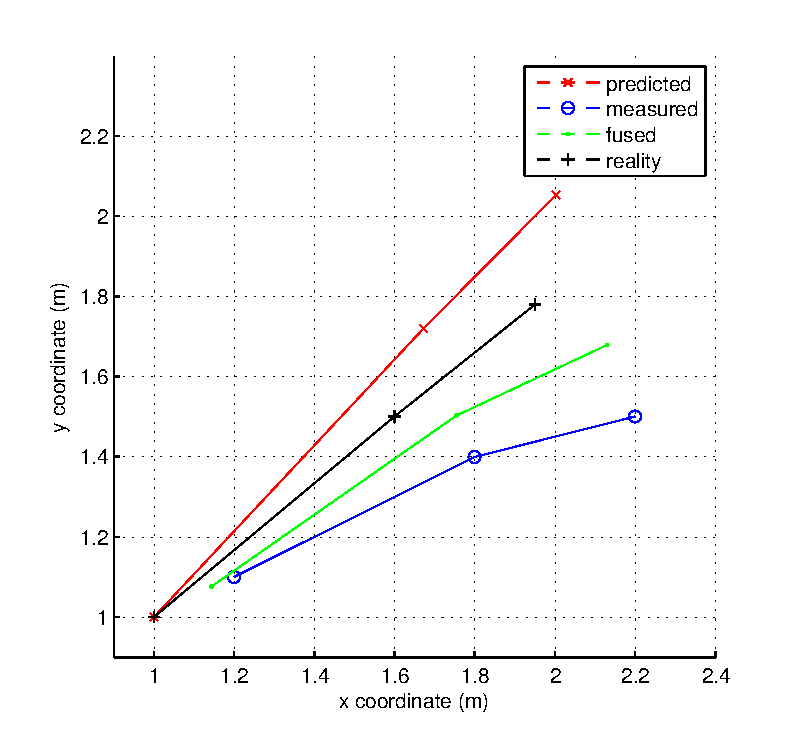
\includegraphics[width=0.7\textwidth]{figs/CONTROLS_Kalman_2D_example.pdf}
\end{figure}
\vspace{-0.18in}
The MSE for prediction    : 0.36\\
The MSE for measurements  : 0.44\\
The MSE for fused estimate: 0.28\\
The advantage of the Kalman filter is that the fused estimate it produces has least error as compared to predicted and measured values.
\end{frame}


%-------
\subsubsection{Proof}
%-------
\begin{frame}\pw\Large
\frametitle{Kalman Filter/Observer/Estimator}
\framesubtitle{Product of Gaussian distributions is a Gaussian function}

\footnotetext{\tiny\hspace{-0.23in} \hspace{-0.25in}
\href{http://blog.jafma.net/2010/11/09/the-product-of-two-Gaussian-pdfs-is-not-a-pdf-but-is-Gaussian-a-k-a-loving-algebra/}{http://blog.jafma.net/2010/11/09/the-product-of-two-Gaussian-pdfs-is-not-a-pdf-but-is-Gaussian-a-k-a-loving-algebra/}}

%\begin{figure}
%\centering
%\includegraphics[width=1.3\textwidth]{figs/BOOK_Dorf_Eg_13_3.pdf}
%\end{figure}
\scriptsize
\begin{equation*}
\begin{array}{llll}
\multicolumn{2}{l}{\textrm{Let $p_1$ and $p_2$ be two Gaussian pdfs with the same support:}}\\\\
p_1(x; \muone, \sone)&=\frac{1}{\sqrt{2 \pi \varone}} e^{-\frac{(x-\muone)^2}{2 \varone}}\\
p_2(x; \mutwo, \stwo)&=\frac{1}{\sqrt{2 \pi \vartwo}} e^{-\frac{(x-\mutwo)^2}{2 \vartwo}}\\\\

\multicolumn{2}{l}{\textrm{Their product is,}}\\
p_1p_2 &=     \frac{1}{\sqrt{2 \pi \varone}} e^{-\frac{(x-\muone)^2}{2 \varone}}    \frac{1}{\sqrt{2 \pi \vartwo}} e^{-\frac{(x-\mutwo)^2}{2 \vartwo}}\\\\
\end{array}
\end{equation*}
%
\end{frame}




\begin{frame}\pw\Large
\frametitle{Kalman Filter/Observer/Estimator}
\framesubtitle{Product of Gaussian distributions is a Gaussian function}

\footnotetext{\tiny\hspace{-0.23in} \hspace{-0.25in}
\href{http://blog.jafma.net/2010/11/09/the-product-of-two-Gaussian-pdfs-is-not-a-pdf-but-is-Gaussian-a-k-a-loving-algebra/}{http://blog.jafma.net/2010/11/09/the-product-of-two-Gaussian-pdfs-is-not-a-pdf-but-is-Gaussian-a-k-a-loving-algebra/}}

%\begin{figure}
%\centering
%\includegraphics[width=1.3\textwidth]{figs/BOOK_Dorf_Eg_13_3.pdf}
%\end{figure}
\scriptsize
\begin{equation*}
\begin{array}{llll}



\multicolumn{2}{l}{\textrm{combining exponents,}}\\
&=\frac{1}{\sqrt{2 \pi \varone \vartwo 2 \pi }}         e^{ -\frac{(x-\muone)^2}{2 \varone} - \frac{(x-\mutwo)^2}{2 \vartwo} } \\\\

\multicolumn{2}{l}{\textrm{taking LCM,}}\\
&=    \frac{1}{\sqrt{2 \pi \varone \vartwo 2 \pi }}         e^{ \frac{ - \vartwo (x-\muone)^2 - \varone (x-\mutwo)^2 } { 2 \varone \vartwo } }\\


\end{array}
\end{equation*}
%
\end{frame}






\begin{frame}\pw\Large
\frametitle{Kalman Filter/Observer/Estimator}
\framesubtitle{Product of Gaussian distributions is a Gaussian function}

\footnotetext{\tiny\hspace{-0.23in} \hspace{-0.25in}
\href{http://blog.jafma.net/2010/11/09/the-product-of-two-Gaussian-pdfs-is-not-a-pdf-but-is-Gaussian-a-k-a-loving-algebra/}{http://blog.jafma.net/2010/11/09/the-product-of-two-Gaussian-pdfs-is-not-a-pdf-but-is-Gaussian-a-k-a-loving-algebra/}}

%\begin{figure}
%\centering
%\includegraphics[width=1.3\textwidth]{figs/BOOK_Dorf_Eg_13_3.pdf}
%\end{figure}
\scriptsize

\begin{equation*}
\begin{array}{llllllll}
\multicolumn{2}{l}{\textrm{Multiply and divide by ${ \varone + \vartwo }$.  This is possible because}}\\
\multicolumn{2}{l}{\textrm{ ${ \varone + \vartwo } > 0$ (otherwise we would be talking about the product of}}\\
\multicolumn{2}{l}{\textrm{ two Dirac delta functions, which would be 0 unless $\muone = \mutwo$)}}\\

p_1 p_2 &=    \frac{1}{\sqrt{2 \pi \frac { \varone \vartwo }{\varone + \vartwo} ( \varone + \vartwo ) 2 \pi }}         e^{ \xx}\\\\

\multicolumn{2}{l}{\textrm{Now we can separate $\frac{1}{\sqrt{2 \pi ( \varone + \vartwo ) }}$ from the non-exponent part }}\\
\multicolumn{2}{l}{\textrm{which resembles the scale factor of a Gaussian pdf,}}\\
\multicolumn{2}{l}{\textrm{and then raise it to $e^{\ln}$,}}\\
p_1 p_2 &=    \frac{1}{\sqrt{2 \pi \frac { \varone \vartwo }{\varone + \vartwo} }}     \frac{1}{\sqrt{2 \pi ( \varone + \vartwo ) }}         e^{ \xx}\\

&=\frac{1}{\sqrt{2 \pi \frac { \varone \vartwo }{\varone + \vartwo} }}     e^{ \ln { \frac{1}{\sqrt{2 \pi ( \varone + \vartwo ) }} }  }        e^{ \xx}\\
\end{array}
\end{equation*}
%
\end{frame}





\begin{frame}\pw\Large
\frametitle{Kalman Filter/Observer/Estimator}
\framesubtitle{Product of Gaussian distributions is a Gaussian function}

\footnotetext{\tiny\hspace{-0.23in} \hspace{-0.25in}
\href{http://blog.jafma.net/2010/11/09/the-product-of-two-Gaussian-pdfs-is-not-a-pdf-but-is-Gaussian-a-k-a-loving-algebra/}{http://blog.jafma.net/2010/11/09/the-product-of-two-Gaussian-pdfs-is-not-a-pdf-but-is-Gaussian-a-k-a-loving-algebra/}}

%\begin{figure}
%\centering
%\includegraphics[width=1.3\textwidth]{figs/BOOK_Dorf_Eg_13_3.pdf}
%\end{figure}
\scriptsize

\begin{equation*}
\begin{array}{llllllll}
\multicolumn{2}{l}{\textrm{Combine exponents,}}\\
&=\frac{1}{\sqrt{2 \pi \frac { \varone \vartwo }{\varone + \vartwo} }}     e^{ \ln { \frac{1}{\sqrt{2 \pi ( \varone + \vartwo ) }} }  +           \xx}\\\\

\multicolumn{2}{l}{\textrm{replace square root in denominator of ln with -1/2,}}\\
&=\frac{1}{\sqrt{2 \pi \frac { \varone \vartwo }{\varone + \vartwo} }}     e^{  - \frac{1}{2} \myalpha  +           \xx}\\\\

\multicolumn{2}{l}{\textrm{Ok, it is time to focus only on the exponent of $e$.}}\\ 
\multicolumn{2}{l}{\textrm{Take LCM,}}\\

&\frac        { - {\color{darkgreen}( \frac { \varone \vartwo }{\varone + \vartwo})} \myalpha              - {\color{darkgreen}\frac { \vartwo }{\varsum} (x-\muone)^2 - \frac{ \varone }{\varsum} (x-\mutwo)^2          }}          {             {\color{darkgreen}2 \frac { \varprod }{\varsum}}} 
\end{array}
\end{equation*}
%
\end{frame}







\begin{frame}[plain]\pw\Large
\frametitle{Kalman Filter/Observer/Estimator}
\framesubtitle{Product of Gaussian distributions is a Gaussian function}

\footnotetext{\tiny\hspace{-0.23in} \hspace{-0.25in}
\href{http://blog.jafma.net/2010/11/09/the-product-of-two-Gaussian-pdfs-is-not-a-pdf-but-is-Gaussian-a-k-a-loving-algebra/}{http://blog.jafma.net/2010/11/09/the-product-of-two-Gaussian-pdfs-is-not-a-pdf-but-is-Gaussian-a-k-a-loving-algebra/}}

%\begin{figure}
%\centering
%\includegraphics[width=1.3\textwidth]{figs/BOOK_Dorf_Eg_13_3.pdf}
%\end{figure}
\scriptsize

\begin{equation*}
\begin{array}{llllllll}
\multicolumn{2}{l}{\textrm{Then we expand the square terms that include $x$ and let ${\color{red}\alpha}=\myalpha$,}}\\ 

&\frac        {             - {\color{darkgreen}( \frac { \varone \vartwo }{\varone + \vartwo})} {\color{red}\alpha}              - {\color{darkgreen}\frac { \vartwo }{\varone + \vartwo} (x^2+\muone^2-2x\muone) - \frac{ \varone }{\varone + \vartwo} (x^2+\mutwo^2-2x\mutwo)  }        }          { \divvarprodvarsum}\\\\

\multicolumn{2}{l}{\textrm{And then we collect the numerator as a polynomial in $x$:}}\\ 

&=\frac        {            {\color{darkgreen}x^2 ( \frac {- \varone - \vartwo }{ \varone + \vartwo } )            - 2 ( \frac {- \muone \vartwo - \mutwo \varone }{ \varone + \vartwo} )x            +} ( \frac { {\color{darkgreen}- {\muone}^2 \vartwo - {\mutwo}^2 \varone - \varone \vartwo} {\color{red}\alpha}}{\color{darkgreen} \varone + \vartwo } )         }         {\divvarprodvarsum}\\\\

&=\frac        {       {\color{darkgreen}- x^2            + 2 ( \frac { \muone \vartwo + \mutwo \varone }{ \varone + \vartwo} )x            -} ( \frac {  {\color{darkgreen}{\muone}^2 \vartwo + {\mutwo}^2 \varone + \varone \vartwo} {\color{red}\alpha} }{\color{darkgreen} \varone + \vartwo } )         }         {\divvarprodvarsum}\\\\
&=\frac{-x^2+2Ax-(A^2+C)}{ \divvarprodvarsum}\\\\
&=\frac{-(x-A)^2-C}{ \divvarprodvarsum}\\
\end{array}
\end{equation*}

\end{frame}



\begin{frame}[plain]\pw\Large
\frametitle{Kalman Filter/Observer/Estimator}
\framesubtitle{Product of Gaussian distributions is a Gaussian function}

\footnotetext{\tiny\hspace{-0.23in} \hspace{-0.25in}
\href{http://blog.jafma.net/2010/11/09/the-product-of-two-Gaussian-pdfs-is-not-a-pdf-but-is-Gaussian-a-k-a-loving-algebra/}{http://blog.jafma.net/2010/11/09/the-product-of-two-Gaussian-pdfs-is-not-a-pdf-but-is-Gaussian-a-k-a-loving-algebra/}}

\scriptsize
%A polynomial of the form $-x^2+2Ax-(A^2+C)$ turns out to be equivalent to \\$-(x-A)^2-C$, which is the form of the exponent of an unidimensional Gaussian pdf plus a constant term. Casually, we had in the above expresion that polynomial if we do:
%
%We are just a few steps from knowing how close is our product of Gaussian pdfs to yield another Gaussian pdf! But first, let us take a short detour to obtain the value of C in our expression:
\begin{equation*}
\begin{array}{rlllllll}
\multicolumn{2}{l}{\textrm{where,}}\\ 
A&={\color{darkgreen}\frac { \muone \vartwo + \mutwo \varone }{ \varone + \vartwo}}\ \ \ {\textrm{and}}\ \ \ A^2+C=\frac {  {\color{darkgreen}{\muone}^2 \vartwo + {\mutwo}^2 \varone + \varone \vartwo} {\color{red}\alpha} }{\color{darkgreen} \varone + \vartwo }\\\\
\multicolumn{2}{l}{\textrm{Then,}}\\ 
C&=\frac {  {\color{darkgreen}{\muone}^2 \vartwo + {\mutwo}^2 \varone + \varone \vartwo} {\color{red}\alpha} }{\color{darkgreen} \varone + \vartwo } - A^2\\
&=\frac {  {\color{darkgreen}{\muone}^2 \vartwo + {\mutwo}^2 \varone + \varone \vartwo} {\color{red}\alpha} }{\color{darkgreen} \varone + \vartwo } -     ({\color{darkgreen}\frac { \muone \vartwo + \mutwo \varone }{ \varone + \vartwo}})^2\\
&=\frac  {      ( {\muone}^2 \vartwo + {\mutwo}^2 \varone + \varone \vartwo {\color{red}\alpha} ) (\varone + \vartwo) -      (\muone \vartwo + \mutwo \varone)^2  }  {      (\varone + \vartwo)^2  }\\
&=\frac  {      {\muone}^2 {\stwo}^4 + {\mutwo}^2 \varone \vartwo + \varone {\stwo}^4 {\color{red}\alpha} + {\muone}^2 \vartwo \varone + {\mutwo}^2 {\sone}^4 + {\sone}^4 \vartwo {\color{red}\alpha} - {\muone}^2 {\stwo}^4 - {\mutwo}^2 {\sone}^4 - 2{\muone}{\mutwo} \varone \vartwo  }  {      (\varone + \vartwo)^2  }\\
&=\frac  {      {\mutwo}^2 \varone \vartwo + \varone {\stwo}^4 {\color{red}\alpha} + {\muone}^2 \vartwo \varone + {\sone}^4 \vartwo {\color{red}\alpha} - 2{\muone}{\mutwo} \varone \vartwo  }  {      (\varone + \vartwo)^2  }\\
&=\frac  {      \varone \vartwo ( {\mutwo}^2 + \vartwo {\color{red}\alpha} + {\muone}^2 + \varone {\color{red}\alpha} - 2{\muone}{\mutwo} )  }   {      (\varone + \vartwo)^2  }\\
&=\frac  {      \varone \vartwo ( ( {\muone} - {\mutwo} )^2 + (\varone + \vartwo) {\color{red}\alpha} )  }   {      (\varone + \vartwo)^2  }\\
&=\frac { \varone \vartwo }{ (\varone + \vartwo)^2 } ({\muone} - {\mutwo} )^2+\frac { \varone \vartwo }{ \varone + \vartwo } \myalpha )\\
\end{array}
\end{equation*}

\end{frame}




\begin{frame}[plain]\pw\Large
\frametitle{Kalman Filter/Observer/Estimator}
\framesubtitle{Product of Gaussian distributions is a Gaussian function}

\footnotetext{\tiny\hspace{-0.23in} \hspace{-0.25in}
\href{http://blog.jafma.net/2010/11/09/the-product-of-two-Gaussian-pdfs-is-not-a-pdf-but-is-Gaussian-a-k-a-loving-algebra/}{http://blog.jafma.net/2010/11/09/the-product-of-two-Gaussian-pdfs-is-not-a-pdf-but-is-Gaussian-a-k-a-loving-algebra/}}

\scriptsize
Ook. We have already values for $A$ and $C$. Using those letters, the resulting product of the two Gaussian pdfs has become:
\begin{equation*}
\begin{array}{rlllllll}
p_1p_2&=    \frac{1}{\sqrt{2 \pi \frac { \varone \vartwo }{\varone + \vartwo} }}    e^{ \frac{-(x-A)^2-C}{2 \frac{\varone \vartwo}{\varone + \vartwo}} } \\
&=    \frac{1}{\sqrt{2 \pi \frac { \varone \vartwo }{\varone + \vartwo} }}    e^{ \frac{-(x-A)^2}{2 \frac{\varone \vartwo}{\varone + \vartwo}} }   e^{- \frac {C}{2 \frac{\varone \vartwo}{\varone + \vartwo}} }
\end{array}
\end{equation*}

\end{frame}




\begin{frame}[plain]\pw\Large
\frametitle{Kalman Filter/Observer/Estimator}
\framesubtitle{Product of Gaussian distributions is a Gaussian function}

\footnotetext{\tiny\hspace{-0.23in} \hspace{-0.25in}
\href{http://blog.jafma.net/2010/11/09/the-product-of-two-Gaussian-pdfs-is-not-a-pdf-but-is-Gaussian-a-k-a-loving-algebra/}{http://blog.jafma.net/2010/11/09/the-product-of-two-Gaussian-pdfs-is-not-a-pdf-but-is-Gaussian-a-k-a-loving-algebra/}}

\scriptsize
Notice that the first factor and the first exponential are a Gaussian pdf. The whole result, however, is just a Gaussian function, unless the second exponential equals 1…

Let us take a closer look to that second exponential, the reason why our result is not a Gaussian pdf but a Gaussian function:
\begin{equation*}
\begin{array}{rlllllll}
e^{- \frac {C}{2 \frac{\varone \vartwo}{\varone + \vartwo}} }&=   e^{- \frac { \frac { \varone \vartwo }{ (\varone + \vartwo)^2 } ({\muone} - {\mutwo} )^2+\frac { \varone \vartwo }{ \varone + \vartwo } \myalpha }        {2 \frac{\varone \vartwo}{\varone + \vartwo}} }\\\\
&=e^{- \frac { ({\muone} - {\mutwo} )^2 }{ 2 (\varone + \vartwo) }         - \frac{1}{2} \myalpha       } \\\\
&=   e^{- \frac { ({\muone} - {\mutwo} )^2 }{ 2( \varone + \vartwo )} }   e^{- \frac{1}{2} \myalpha } \\\\
&= \frac {1}{ \sqrt{2 \pi (\varone + \vartwo)} }   e^{- \frac { ({\muone} - {\mutwo} )^2 }{ 2(\varone + \vartwo) } }
\end{array}
\end{equation*}

\end{frame}





\begin{frame}[plain]\pw\Large
\frametitle{Kalman Filter/Observer/Estimator}
\framesubtitle{Product of Gaussian distributions is a Gaussian function}

\footnotetext{\tiny\hspace{-0.23in} \hspace{-0.25in}
\href{http://blog.jafma.net/2010/11/09/the-product-of-two-Gaussian-pdfs-is-not-a-pdf-but-is-Gaussian-a-k-a-loving-algebra/}{http://blog.jafma.net/2010/11/09/the-product-of-two-Gaussian-pdfs-is-not-a-pdf-but-is-Gaussian-a-k-a-loving-algebra/}}

\scriptsize
Surprisingly, this last expression is a Gaussian pdf if we consider $\muone$ a variable, i.e., $p(\muone; \mutwo, \sqrt{(\varone+\vartwo)})$ (we can also consider $\mutwo$ the variable). But what we are interested in is knowing under which conditions this expression equals 1, and, thus, the product of our original pdfs $p_1$ and $p_2$ is actually a Gaussian pdf:
\begin{equation*}
\begin{array}{rlllllll}
\frac {1}{ \sqrt{2 \pi (\varone + \vartwo)} }   e^{- \frac { ({\muone} - {\mutwo} )^2 }{ 2(\varone + \vartwo) } } = 1  \Leftrightarrow    - \frac { ({\muone} - {\mutwo} )^2 }{ 2(\varone + \vartwo) }   = \ln ( \sqrt{2 \pi (\varone + \vartwo)} )  \Leftrightarrow\\\\
- \frac { ({\muone} - {\mutwo} )^2 }{ 2(\varone + \vartwo) }   = \frac {1}{2} \ln ( 2 \pi (\varone + \vartwo) )  \Leftrightarrow\\\\
-  ({\muone} - {\mutwo} )^2    = (\varone + \vartwo) \ln ( 2 \pi (\varone + \vartwo) ) 
\end{array}
\end{equation*}

\end{frame}




\begin{frame}[plain]\pw\Large
\frametitle{Kalman Filter/Observer/Estimator}
\framesubtitle{Product of Gaussian distributions is a Gaussian function}

\footnotetext{\tiny\hspace{-0.23in} \hspace{-0.25in}
\href{http://blog.jafma.net/2010/11/09/the-product-of-two-Gaussian-pdfs-is-not-a-pdf-but-is-Gaussian-a-k-a-loving-algebra/}{http://blog.jafma.net/2010/11/09/the-product-of-two-Gaussian-pdfs-is-not-a-pdf-but-is-Gaussian-a-k-a-loving-algebra/}}
\scriptsize
Since ${ {\sigma_{1}}^{2} + {\sigma_{2}}^{2} }$ is greater than zero, and the expectations are independent from the variances, we will always find cases (infinite cases, actually) in which the equality does not hold. Thus, we will find infinite cases where the product of two Gaussian pdfs is a Gaussian function but not a Gaussian pdf.

Nevertheless: the scaled Gaussian function obtained as the result of the product has the following pdf-like parameters:
\begin{equation*}
\begin{array}{rlllllll}
A &= \frac { \muone \vartwo + \mutwo \varone }{ \varone + \vartwo}\\\\
{\sigma_{1 x 2}}^2 &= \frac{\varone \vartwo}{\varone + \vartwo}
\end{array}
\end{equation*}

\end{frame}








%\begin{frame}\pw\Large
%\frametitle{Kalman Filter/Observer/Estimator}
%\framesubtitle{An Observer (Estimator): The Kalman Filter}
%
%\footnotetext{\tiny\hspace{-0.23in} \href{http://greg.czerniak.info/guides/kalman1/}{http://greg.czerniak.info/guides/kalman1/}}
%\scriptsize \vspace{0.1in}An example usage of the Kalman filter:
%\begin{figure}[h]
%\centering
%\includegraphics[width=1\textwidth]{figs/CONTROLS_Kalman_canon.pdf}
%\end{figure}
%\end{frame}

\begin{frame}\pw\Large
\frametitle{Kalman Filter/Observer/Estimator}
\framesubtitle{Introduction \tiny cont.}
\footnotetext{\tiny\hspace{-0.23in} \href{http://www.cl.cam.ac.uk/~rmf25/papers/Understanding the Basis of the Kalman Filter.pdf}{Faragher, Ramsey, \emph{Understanding the Basis of the Kalman Filter Via a Simple and Intuitive Derivation}, IEEE Signal Processing Magazine, Sep 2012}}
\begin{itemize}
\item The Kalman filter is over 50 years old but is still one of the most important and common \underline{data fusion} algorithms in use today
\item The great success of the Kalman filter is due to 
\begin{itemize}\scriptsize
\item its small computational requirement
\item elegant recursive properties, and 
\item its status as the optimal estimator for one-dimensional linear systems with Gaussian error statistics
\end{itemize}
\end{itemize}
\end{frame}

\end{document}
